\documentclass[11pt]{article}

\usepackage[utf8]{inputenc}
\usepackage[a4paper,margin=1in]{geometry}
\usepackage{newtxtext}
\usepackage{microtype}
\usepackage{lettrine}
\usepackage{setspace}
\usepackage{enumitem}

% Mathematics
\usepackage{amsmath,amssymb,amsfonts}

% Graphics & Drawing
\usepackage{graphicx}
\usepackage{tikz}
\usepackage{pgfplots}
\usepackage{circuitikz}
\usepackage{smartdiagram}
\usepackage{tikz-3dplot}

% Tables
\usepackage{booktabs}
\usepackage{tabularx}
\usepackage{multirow}
\usepackage{array}
\usepackage{needspace}

% IEEE-style Enhancements
\usepackage{titlesec}
\usepackage{fancyhdr}
\usepackage{caption}
\usepackage{subcaption}
\usepackage{tcolorbox}
\usepackage{mdframed}
\tcbuselibrary{skins,breakable}

% Hyperlinks
\usepackage{hyperref}

% Colors
\usepackage{xcolor}

% Timeline & Shapes
\usetikzlibrary{
arrows.meta,
positioning,
calc,
shapes.geometric,
shapes.symbols,
fit,
backgrounds,
decorations.pathmorphing,
patterns,
3d,
matrix
}

\pgfplotsset{compat=1.18}


% Define IEEE-inspired Professional Color Palette (Blue and Orange)
\definecolor{IEEEblue}{HTML}{003B73}
\definecolor{IEEEorange}{HTML}{F28C28}
\definecolor{SoftBlue}{HTML}{EEF6FF}
\definecolor{SoftOrange}{HTML}{FFF4E8}
\definecolor{DarkGray}{HTML}{222222}
\definecolor{LightGray}{HTML}{F7F9FC}
\definecolor{MidGray}{HTML}{6B7280}
\definecolor{PanelBlue}{HTML}{F5FAFF}
\definecolor{PanelOrange}{HTML}{FFF8EF}

% Setup Hypersetup for elegant links
\hypersetup{
    colorlinks=true,
    linkcolor=IEEEblue,
    citecolor=IEEEorange,
    urlcolor=IEEEblue
}

% Page and section headers/footers styling
\pagestyle{fancy}
\fancyhf{}
\lhead{\footnotesize\color{DarkGray} Neuromorphic Computing}
\rhead{\footnotesize\color{DarkGray} Arjun Mitra}
\cfoot{\footnotesize\color{DarkGray}\thepage}
\renewcommand{\headrulewidth}{0.4pt}
\renewcommand{\headrule}{\hbox to\headwidth{\color{IEEEblue!45}\leaders\hrule height \headrulewidth\hfill}}
\renewcommand{\footrulewidth}{0pt}
\setlength{\headheight}{22pt}
\onehalfspacing
\setlength{\parskip}{0.55em}
\setlength{\parindent}{1.2em}
\renewcommand{\arraystretch}{1.18}
\setlist[itemize]{leftmargin=1.45em,itemsep=0.18em,topsep=0.25em,label=\textcolor{IEEEorange}{\small$\blacktriangleright$}}

% Section formatting
\titleformat{\section}
  {\color{IEEEblue}\normalfont\large\bfseries\scshape}{\colorbox{IEEEblue!88}{\color{white}\strut\thesection}}{0.75em}{}[\vspace{0.5em}{\color{IEEEorange!70}\titlerule[0.55pt]}\vspace{0.8em}]
\titlespacing*{\section}{0pt}{1.15em}{0.25em}
\titleformat{\subsection}
  {\color{IEEEblue}\normalfont\large\bfseries}{\textcolor{IEEEorange}{\rule[-0.15em]{0.18em}{1.05em}}\hspace{0.45em}\thesubsection}{0.65em}{}
\titlespacing*{\subsection}{0pt}{1.0em}{0.35em}

% Caption settings
\captionsetup{font={small,it},labelfont={bf,color=IEEEblue},width=0.9\textwidth,justification=centering,singlelinecheck=false,skip=5pt}
\setlength{\emergencystretch}{3em}

% Decorative drop-cap opening used for major section lead paragraphs
\newcommand{\sectionlead}[2]{\noindent\lettrine[lines=2,lhang=0.08,nindent=0.12em]{\textcolor{IEEEblue}{\bfseries #1}}{\hspace{0.03em}#2}}

% Professional highlight box environments
\newtcolorbox{researchbox}{
    enhanced,
    breakable,
    colback=PanelBlue,
    colframe=IEEEblue,
    arc=2.5mm,
    boxrule=0.8pt,
    borderline west={2.2pt}{0pt}{IEEEblue},
    drop shadow={IEEEblue!18!white},
    left=3mm,
    right=3mm,
    top=2mm,
    bottom=2mm
}

\newtcolorbox{futurebox}{
    enhanced,
    breakable,
    colback=PanelOrange,
    colframe=IEEEorange,
    arc=2.5mm,
    boxrule=0.8pt,
    borderline west={2.2pt}{0pt}{IEEEorange},
    drop shadow={IEEEorange!18!white},
    left=3mm,
    right=3mm,
    top=2mm,
    bottom=2mm
}

\begin{document}
\hypersetup{pageanchor=false}
\pagenumbering{gobble}


\begin{titlepage}
    \centering
    \vspace*{0.35cm}

    \begin{tikzpicture}[remember picture,overlay]
        \fill[IEEEblue!4] (current page.south west) rectangle (current page.north east);
        \fill[IEEEblue] ([yshift=-0.35cm]current page.north west) rectangle ([yshift=-0.62cm]current page.north east);
        \fill[IEEEorange] ([yshift=-0.62cm]current page.north west) rectangle ([yshift=-0.72cm]current page.north east);
        \draw[IEEEblue!28, line width=0.9pt, rounded corners=12pt]
            ([xshift=1.05cm,yshift=-1.05cm]current page.north west) rectangle
            ([xshift=-1.05cm,yshift=1.05cm]current page.south east);
        \draw[IEEEorange!70, line width=1.1pt]
            ([xshift=1.35cm,yshift=-1.35cm]current page.north west) --
            ([xshift=4.2cm,yshift=-1.35cm]current page.north west);
        \draw[IEEEorange!70, line width=1.1pt]
            ([xshift=-1.35cm,yshift=1.35cm]current page.south east) --
            ([xshift=-4.2cm,yshift=1.35cm]current page.south east);
    \end{tikzpicture}

    {\color{IEEEblue}\Large\bfseries Technical Report\par}
    \vspace{0.15cm}
    {\color{IEEEorange}\rule{0.22\textwidth}{1pt}\par}
    \vspace{0.18cm}
    {\color{DarkGray}\small\bfseries St. Thomas' College of Engineering and Technology\par}

    \vspace{0.36cm}

    \begin{tikzpicture}[x=1cm,y=1cm,>=Latex]
        \fill[IEEEblue!5, rounded corners=10pt, draw=IEEEblue!35, line width=0.8pt] (-4.25,-1.78) rectangle (4.25,1.78);
        \fill[white, rounded corners=8pt] (-4.05,-1.58) rectangle (4.05,1.58);
        \node[circle, draw=IEEEblue, fill=SoftBlue, line width=1pt, minimum size=2.35cm] (brain) at (-1.55,0) {};
        \foreach \a in {20,65,115,160,215,260,315}{
            \draw[IEEEblue!70, line width=0.65pt] (brain.center) -- ++(\a:0.95);
            \fill[IEEEorange] ($(brain.center)+(\a:0.95)$) circle (1.3pt);
        }
        \draw[IEEEblue!55, line width=0.9pt]
            (-2.15,0.25) .. controls (-2.35,0.95) and (-1.65,1.1) .. (-1.45,0.55)
            .. controls (-0.85,1.0) and (-0.65,0.25) .. (-1.05,0.05)
            .. controls (-0.55,-0.35) and (-1.2,-1.0) .. (-1.55,-0.55)
            .. controls (-2.0,-1.05) and (-2.45,-0.35) .. (-2.15,0.25);
        \draw[-Latex, line width=1pt, IEEEorange] (-0.2,0) -- (0.82,0);
        \draw[IEEEblue, fill=IEEEblue!8, line width=1pt, rounded corners=2pt] (0.95,-0.85) rectangle (2.65,0.85);
        \foreach \x in {1.15,1.45,...,2.45}{
            \draw[IEEEblue!65, line width=0.45pt] (\x,-1.05) -- (\x,-0.85);
            \draw[IEEEblue!65, line width=0.45pt] (\x,0.85) -- (\x,1.05);
        }
        \foreach \y in {-0.55,-0.25,0.05,0.35,0.65}{
            \draw[IEEEblue!65, line width=0.45pt] (0.75,\y) -- (0.95,\y);
            \draw[IEEEblue!65, line width=0.45pt] (2.65,\y) -- (2.85,\y);
        }
        \node[text=IEEEblue, font=\bfseries\scriptsize, align=center] at (1.8,0) {SNN\\Chip};
        \node[text=MidGray, font=\scriptsize] at (0,-1.35) {Human brain inspiration $\rightarrow$ neuromorphic silicon};
    \end{tikzpicture}

    \vspace{0.55cm}

    \begin{tcolorbox}[
        enhanced,
        colback=white,
        colframe=IEEEblue!70,
        borderline west={3pt}{0pt}{IEEEorange},
        arc=3mm,
        boxrule=0.9pt,
        width=0.91\textwidth,
        left=5mm,
        right=5mm,
        top=4mm,
        bottom=4mm,
        drop shadow={IEEEblue!16!white},
        title={\large\bfseries Article Details},
        coltitle=white,
        colbacktitle=IEEEblue,
        attach boxed title to top center={yshift=-2mm},
        boxed title style={arc=2mm,boxrule=0pt,left=6mm,right=6mm}
    ]
    \renewcommand{\arraystretch}{1.35}
    \begin{tabularx}{\textwidth}{>{\bfseries\color{IEEEblue}}p{3.9cm}X}
        Topic & Neuromorphic Computing Chips Inspired by the Human Brain \\
        Title & \textbf{Brain-Inspired Neuromorphic Computing Chips for Energy-Efficient Artificial Intelligence} \\
        Name & Arjun Mitra \\
        Year & 3rd Year \\
        Class Roll Number & 41 \\
        Department & Electronics and Communication Engineering \\
    \end{tabularx}
    \end{tcolorbox}

    \vspace{0.5cm}

    \begin{tcolorbox}[
        enhanced,
        colback=PanelOrange,
        colframe=IEEEorange!85,
        arc=2.5mm,
        boxrule=0.75pt,
        width=0.82\textwidth,
        left=4mm,
        right=4mm,
        top=2.5mm,
        bottom=2.5mm
    ]
    \centering\small\itshape
    Submitted as part of the celebration of National Technology Day.
    \end{tcolorbox}
    
    \vfill
\end{titlepage}

\clearpage
\hypersetup{pageanchor=true}
\pagenumbering{roman}
\setcounter{page}{1}

\begin{titlepage}
    \thispagestyle{plain}
    \begin{center}
        \null
        \vspace{1.2cm}
        {\color{IEEEblue}\LARGE\bfseries Abstract\par}
        \vspace{0.25cm}
        {\color{IEEEorange}\rule{0.22\textwidth}{0.8pt}\par}
    \end{center}
    \vspace{0.45cm}

    \begin{abstract}
    The rise of modern deep learning has highlighted severe limitations within the traditional Von Neumann computer architecture, primarily governed by memory transfer bottlenecks and unsustainable power requirements. Neuromorphic architectures utilize Spiking Neural Networks (SNNs) to represent information as sparse, asynchronous temporal spikes, co-locating processing and memory within physical neuron and synapse models. This paper analyzes the core mathematical principles of SNNs, details the microelectronic physics of memristive devices representing physical synapses, and contrasts state-of-the-art brain-inspired hardware platforms, including IBM TrueNorth, Intel Loihi 1 \& 2, SpiNNaker 1 \& 2, and the brain-scale Intel Hala Point chassis. Furthermore, it discusses edge AI and robotic applications that demonstrate major gains in energy-delay product. Emerging frontiers such as integrated photonic neuromorphic circuits and quantum neuromorphic frameworks are reviewed alongside systematic bottlenecks, highlighting the technological roadmap for post-Moore computing.
    \end{abstract}

    \vfill
\end{titlepage}

\clearpage
\setcounter{page}{2}
\tableofcontents
\clearpage
\listoffigures
\clearpage
\listoftables
\clearpage
\pagenumbering{arabic}
\setcounter{page}{1}

%=============================================================================
% MAIN CONTENT
%=============================================================================

\section{Introduction}
\sectionlead{M}{odern artificial intelligence has experienced an exponential explosion in computing requirements}, driving massive deployments of deep neural network architectures \cite{schuman2017survey}. However, executing these dense models on conventional silicon processors is increasingly constrained by the "power wall" and the classical Von Neumann bottleneck, where constant data shuttling between discrete memory and processing units dissipates up to 90\% of system energy \cite{schuman2017survey}. The biological human brain, by contrast, executes highly sophisticated cognitive, sensory, and motor tasks on an energy budget of roughly 20 W \cite{schuman2017survey,mead1990neuromorphic}. 

Neuromorphic computing, a paradigm first conceived by Carver Mead in the late 1980s, seeks to emulate the structural, functional, and biophysical characteristics of biological neural circuits in custom microelectronics \cite{schuman2017survey,mead1990neuromorphic}. By co-locating computational logic and memory inside silicon-based neural structures, neuromorphic chips completely bypass the Von Neumann bottleneck \cite{schuman2017survey,mead1990neuromorphic}. Leveraging Spiking Neural Networks (SNNs), these systems process information as sparse, asynchronous, event-driven temporal spikes rather than dense, continuous numeric representations \cite{schuman2017survey,mead1990neuromorphic}. This paradigm shift transitions AI hardware from passive, clock-driven calculations to highly efficient, active physical emulations of cognitive intelligence \cite{schuman2017survey,mead1990neuromorphic}.

This report details the architectural, mathematical, and materials-science frameworks that govern neuromorphic chips. Section 2 establishes the structural comparison between Von Neumann and neuromorphic computing. Section 3 outlines the mathematical models of SNNs. Section 4 presents synaptic plasticity, while Section 5 details state-of-the-art chips. Section 6 and Section 7 discuss memristors and real-world edge AI and robotic use cases, and Section 8 highlights emerging photonic and quantum paradigms.


\begin{figure}[htbp]
    \centering
    \resizebox{0.96\textwidth}{!}{%
    \begin{tikzpicture}[
        node distance=0.75cm,
        every node/.style={font=\small\bfseries, align=center},
        motivation/.style={draw, rounded corners=3pt, minimum width=3.05cm, minimum height=1.15cm, inner sep=4pt}
    ]
        \node[motivation, fill=red!10] (gpu) {AI Power\\Crisis};
        \node[motivation, fill=orange!15, right=of gpu] (memory) {Memory\\Bottleneck};
        \node[motivation, fill=blue!10, right=of memory] (brain) {Brain\\Inspiration};
        \node[motivation, fill=green!10, right=of brain] (neuro) {Neuromorphic\\AI};

        \draw[-Latex, thick, IEEEorange] (gpu) -- (memory);
        \draw[-Latex, thick, IEEEorange] (memory) -- (brain);
        \draw[-Latex, thick, IEEEorange] (brain) -- (neuro);
    \end{tikzpicture}%
    }
    \caption{Motivation behind neuromorphic computing development.}
    \label{fig:research_motivation}
\end{figure}

\begin{figure}[htbp]
    \centering
    \resizebox{0.80\textwidth}{!}{%
    \begin{tikzpicture}[node distance=1.5cm, every node/.style={font=\scriptsize}]
        % Traditional Architecture (Von Neumann)
        \draw[thick, IEEEblue, fill=IEEEblue!5] (-3.5, 1.5) rectangle (-1.0, 3.5);
        \node[align=center, text width=2.1cm] at (-2.25, 2.8) {\textbf{Von Neumann}\\\textbf{Processor}\\\textbf{(CPU/GPU)}};
        \draw[thick, IEEEblue, fill=IEEEblue!5] (-3.5, -1.5) rectangle (-1.0, -0.5);
        \node[align=center, text width=2.5cm] at (-2.25, -1.0) {\textbf{Memory}\\\textbf{SRAM/DRAM}};
        
        \draw[<->, >=Latex, line width=1.5pt, IEEEorange] (-2.25, -0.5) -- (-2.25, 1.5) 
            node[midway, right, align=left, text width=2.2cm, text=IEEEorange] {\textbf{Von Neumann}\\\textbf{Bottleneck}\\\textbf{Data Shuttling}};

        % Neuromorphic Architecture
        \draw[thick, IEEEorange, fill=IEEEorange!5] (1.5, -1.5) rectangle (5.5, 3.5);
        \node[above, font=\small\bfseries, text=IEEEblue, text width=4.2cm, align=center] at (3.5, 3.5) {Neuromorphic Grid (In-Memory)};
        
        % Sub-grid of co-located neurocores
        \foreach \x in {2.0, 3.5, 5.0} {
            \foreach \y in {-1.0, 1.0, 2.5} {
                \draw[thick, IEEEblue, fill=IEEEblue!10] (\x-0.3, \y-0.3) rectangle (\x+0.3, \y+0.3);
                \node at (\x, \y) [scale=0.7] {\textbf{C}};
            }
        }
        % Connect the cores (NoC Router mesh)
        \draw[thick, dashed, IEEEblue] (2.0, -1.0) -- (5.0, -1.0);
        \draw[thick, dashed, IEEEblue] (2.0, 1.0) -- (5.0, 1.0);
        \draw[thick, dashed, IEEEblue] (2.0, 2.5) -- (5.0, 2.5);
        \draw[thick, dashed, IEEEblue] (2.0, -1.0) -- (2.0, 2.5);
        \draw[thick, dashed, IEEEblue] (3.5, -1.0) -- (3.5, 2.5);
        \draw[thick, dashed, IEEEblue] (5.0, -1.0) -- (5.0, 2.5);
        
        \node[align=center, text width=3.2cm, text=IEEEblue] at (3.5, -1.8) {\textbf{Asynchronous}\\\textbf{NoC Mesh}};
        
    \end{tikzpicture}%
    }
    \caption{Architectural shift from separated processor--memory data movement to co-located neuromorphic cores with integrated compute and synaptic storage \cite{schuman2017survey,mead1990neuromorphic}.}
    \label{fig:vn_vs_neuromorphic}
\end{figure}

\section{The Biological Paradigm vs. Von Neumann Architectures}
\sectionlead{T}{o achieve high-efficiency cognitive computation, neuromorphic chips transition away} from the central-processing/peripheral-storage separation of Von Neumann machines \cite{schuman2017survey}. In biological brains, processing is inherently decentralized, massively parallel, and self-organizing \cite{schuman2017survey,mead1990neuromorphic}. Memory is represented dynamically by the physical conductance of trillions of synaptic connections \cite{schuman2017survey}. Table~\ref{tab:vn_vs_brain} highlights the fundamental structural differences.

\begin{table}[htbp]
    \centering
    \caption{Key Structural Differences: Von Neumann vs. Human Brain Paradigms \cite{schuman2017survey,mead1990neuromorphic,kudithipudi2025scale}}
    \resizebox{\textwidth}{!}{%
    \begin{tabular}{lll}
        \toprule
        \textbf{Parameter} & \textbf{Von Neumann Architecture} & \textbf{Biological Human Brain} \\
        \midrule
        \textbf{Control Flow} & Centralized, synchronous global clock & Decentralized, fully asynchronous events \\
        \textbf{Memory and Compute} & Separated (CPU/GPU and DRAM) & Integrated (Co-located Synapse/Neuron) \\
        \textbf{Signal Representation} & High-precision, high-frequency bits & Sparse, low-frequency electrical spikes \\
        \textbf{Power Consumption} & Kilowatts to Megawatts (highly active) & Approximately 20 W metabolic budget \\
        \textbf{Structural Scale} & Two-dimensional coplanar silicon & Three-dimensional highly packed volumes \\
        \textbf{Fault Tolerance} & Low (Single-point transistor faults fatal) & High (Graceful degradation via plasticity) \\
        \bottomrule
    \end{tabular}%
    }
    \label{tab:vn_vs_brain}
\end{table}

Traditional architectures require active power continuously because silicon transistors are clocked synchronously to maintain state. Neuromorphic chips, by contrast, use event-driven execution \cite{schuman2017survey,mead1990neuromorphic}. If an incoming sensor stream remains unchanged, no action potentials are fired, reducing active dynamic power to nearly zero.


\begin{table}[htbp]
    \centering
    \caption{Comparison of AI Hardware Architectures}
    \begin{tabular}{lcccc}
        \toprule
        \textbf{Hardware} & \textbf{Power} & \textbf{Parallelism} & \textbf{Learning} & \textbf{Edge AI} \\
        \midrule
        CPU & High & Low & Moderate & Poor \\
        GPU & Very High & Massive & Excellent & Moderate \\
        TPU & High & Massive & Excellent & Moderate \\
        FPGA & Medium & High & Flexible & Good \\
        Neuromorphic & Ultra Low & Massive & Event-driven & Excellent \\
        \bottomrule
    \end{tabular}
    \label{tab:ai_hardware_comparison}
\end{table}

\section{Spiking Neural Network Fundamentals}
\sectionlead{S}{piking Neural Networks represent the third generation of neural network models}, enhancing computational expressiveness by utilizing the temporal properties of information \cite{schuman2017survey}.



\begin{figure}[htbp]
    \centering
    \resizebox{0.94\textwidth}{!}{%
    \begin{tikzpicture}[
        neuron/.style={line cap=round, line join=round},
        trunk/.style={neuron, line width=1.55pt, IEEEblue!78},
        branch/.style={neuron, line width=0.95pt, IEEEblue!68},
        twig/.style={neuron, line width=0.55pt, IEEEblue!58},
        axon/.style={neuron, line width=2.3pt, IEEEblue!90},
        label/.style={font=\small\bfseries, text=DarkGray}
    ]
        % Soft microscope-slide backdrop
        \fill[SoftBlue, rounded corners=10pt] (-4.85,-2.55) rectangle (7.45,2.75);
        \draw[IEEEblue!12, rounded corners=10pt] (-4.85,-2.55) rectangle (7.45,2.75);

        % Dense dendritic arbor around the soma: primary trunks, secondary branches, and tiny spines
        \draw[trunk] (-0.72,0.58) .. controls (-1.30,1.10) and (-2.05,1.55) .. (-3.02,2.15);
        \draw[branch] (-1.28,1.10) .. controls (-1.82,1.62) .. (-2.32,2.35);
        \draw[twig] (-1.72,1.48) .. controls (-1.42,1.95) .. (-1.28,2.42);
        \draw[twig] (-2.26,1.78) .. controls (-2.88,1.62) .. (-3.62,1.68);
        \draw[twig] (-2.75,1.98) .. controls (-3.25,2.38) .. (-3.98,2.46);

        \draw[trunk] (-0.92,0.20) .. controls (-1.68,0.44) and (-2.55,0.28) .. (-3.85,0.78);
        \draw[branch] (-1.74,0.35) .. controls (-2.18,0.92) .. (-2.90,1.18);
        \draw[twig] (-2.35,0.40) .. controls (-3.08,0.18) .. (-4.22,0.08);
        \draw[twig] (-3.10,0.62) .. controls (-3.58,1.15) .. (-4.28,1.28);
        \draw[twig] (-3.42,0.74) .. controls (-3.88,0.52) .. (-4.46,0.58);

        \draw[trunk] (-0.85,-0.30) .. controls (-1.68,-0.80) and (-2.55,-0.88) .. (-3.80,-1.55);
        \draw[branch] (-1.58,-0.72) .. controls (-1.95,-1.28) .. (-2.62,-1.86);
        \draw[twig] (-2.30,-0.98) .. controls (-3.05,-0.78) .. (-3.92,-0.88);
        \draw[twig] (-2.92,-1.28) .. controls (-3.48,-1.84) .. (-4.28,-2.08);
        \draw[twig] (-3.25,-1.42) .. controls (-3.56,-1.18) .. (-4.05,-1.18);

        \draw[trunk] (-0.32,0.86) .. controls (-0.82,1.45) and (-1.02,1.95) .. (-1.58,2.48);
        \draw[branch] (-0.80,1.54) .. controls (-0.45,2.02) .. (-0.36,2.48);
        \draw[twig] (-1.05,1.92) .. controls (-1.64,2.08) .. (-2.04,2.52);

        \draw[trunk] (-0.18,-0.88) .. controls (-0.52,-1.38) and (-0.86,-1.78) .. (-1.55,-2.22);
        \draw[branch] (-0.78,-1.58) .. controls (-0.42,-2.02) .. (-0.20,-2.42);
        \draw[twig] (-1.02,-1.82) .. controls (-1.62,-2.05) .. (-2.18,-2.40);

        % Small dendritic spines for a more biological silhouette
        \foreach \x/\y in {-3.78/1.66,-3.22/2.37,-2.04/2.34,-4.16/1.26,-4.30/0.08,-3.84/-0.88,-4.22/-2.06,-2.12/-2.36,-0.28/-2.38,-0.36/2.44} {
            \fill[IEEEblue!65] (\x,\y) circle (0.035);
        }

        % Irregular soma and nucleus with a more cell-like outline
        \shade[ball color=IEEEorange!32, draw=IEEEorange!80, line width=1pt]
            (0.02,0.86)
            .. controls (0.62,0.86) and (1.10,0.48) .. (1.16,-0.08)
            .. controls (1.22,-0.72) and (0.68,-1.02) .. (0.12,-0.94)
            .. controls (-0.48,-0.86) and (-1.00,-0.52) .. (-0.98,0.10)
            .. controls (-0.96,0.62) and (-0.48,0.90) .. (0.02,0.86) -- cycle;
        \shade[ball color=IEEEblue!25, draw=IEEEblue!65, line width=0.6pt] (0.10,0.02) circle (0.33);
        \fill[white!45, opacity=0.35] (-0.23,0.36) ellipse (0.22 and 0.10);

        % Axon hillock and longer axon with myelin gaps (nodes of Ranvier)
        \filldraw[fill=IEEEorange!35, draw=IEEEorange!85, line width=0.7pt]
            (0.98,0.18) .. controls (1.25,0.10) and (1.46,0.04) .. (1.62,0.00)
            .. controls (1.42,-0.06) and (1.22,-0.16) .. (0.95,-0.24) -- cycle;
        \draw[axon] (1.46,0.00) .. controls (2.15,0.20) and (2.75,-0.18) .. (3.45,0.03)
                         .. controls (4.10,0.22) and (4.82,-0.18) .. (5.42,0.04)
                         .. controls (5.88,0.20) and (6.15,0.05) .. (6.38,0.00);
        \foreach \x/\y/\rot in {1.85/0.06/9,2.45/-0.03/-8,3.05/0.04/7,3.66/-0.02/-7,4.28/0.04/7,4.88/-0.03/-8,5.48/0.04/8} {
            \begin{scope}[shift={(\x,\y)}, rotate=\rot]
                \filldraw[fill=SoftOrange, draw=IEEEorange!75, line width=0.75pt, rounded corners=2pt]
                    (-0.22,-0.24) rectangle (0.22,0.24);
            \end{scope}
        }

        % Rich axon terminal arbor with bouton-like endpoints
        \draw[axon] (6.38,0.00) .. controls (6.62,0.26) and (6.80,0.56) .. (7.08,0.90);
        \draw[axon] (6.38,0.00) .. controls (6.70,0.10) and (6.98,0.08) .. (7.25,0.16);
        \draw[axon] (6.38,0.00) .. controls (6.66,-0.24) and (6.88,-0.55) .. (7.08,-0.92);
        \draw[branch] (7.08,0.90) .. controls (7.24,1.06) .. (7.34,1.26);
        \draw[branch] (7.08,0.90) .. controls (7.32,0.82) .. (7.52,0.74);
        \draw[branch] (7.08,-0.92) .. controls (7.26,-1.10) .. (7.45,-1.28);
        \draw[branch] (7.08,-0.92) .. controls (7.34,-0.82) .. (7.55,-0.72);
        \foreach \p in {(7.36,1.31),(7.58,0.72),(7.31,0.16),(7.50,-1.33),(7.60,-0.70)} {
            \shade[ball color=IEEEorange!60, draw=IEEEorange!90] \p circle (0.105);
        }

        % Direction of spike propagation
        \draw[-Latex, thick, IEEEorange] (2.10,0.68) -- node[above, font=\scriptsize\bfseries, text=IEEEorange] {action potential} (5.62,0.68);

        % Labels
        \node[label] at (-3.12,2.58) {Highly branched dendrites};
        \node[label] at (0,-1.45) {Soma};
        \node[label] at (0.13,0.55) {\scriptsize Nucleus};
        \node[label] at (3.85,-0.78) {Myelinated axon};
        \node[label] at (6.88,1.62) {Synaptic boutons};
    \end{tikzpicture}%
    }
    \caption{Biological neuron structure inspiring neuromorphic systems, with branched dendrites for input collection, soma integration, myelinated axonal transmission, and synaptic bouton outputs.}
    \label{fig:biological_neuron}
\end{figure}


\subsection{Information Representation: Rate vs. Temporal Coding}
Unlike deep neural networks (DNNs) that utilize dense, continuous floating-point values as activation levels, SNNs communicate via discrete binary events called action potentials or "spikes" \cite{schuman2017survey,mead1990neuromorphic}:
$$S_i(t) = \sum_f \delta(t - t_i^{(f)})$$
where $\delta(t)$ represents the Dirac delta function and $t_i^{(f)}$ is the specific arrival time of spike $f$ from neuron $i$ \cite{davies2018loihi}. 

The neuromorphic community characterizes spike-based data representation into two primary paradigms \cite{schuman2017survey,mead1990neuromorphic}:
\begin{enumerate}
    \item \textbf{Rate Coding:} Information is represented as the mean frequency of spikes over an observation window, often modeled via a Poisson process \cite{schuman2017survey,mead1990neuromorphic}. While mathematically simple, rate coding suffers from latency overheads and high spike counts \cite{schuman2017survey,mead1990neuromorphic}.
    \item \textbf{Temporal Coding / Time-to-First-Spike (TTFS):} Information is encoded directly in the precise millisecond-scale latency of a single spike relative to a synchronization event \cite{schuman2017survey,mead1990neuromorphic}. Neurons receiving highly intense stimuli fire first, enabling extremely high-speed, sparse decision-making using a fraction of the power of rate coding \cite{schuman2017survey,mead1990neuromorphic}.
\end{enumerate}

\subsection{The Leaky Integrate-and-Fire (LIF) Mathematical Model}
The leaky integrate-and-fire (LIF) model balances biological accuracy with VLSI microelectronic feasibility \cite{schuman2017survey,mead1990neuromorphic}. A single LIF neuron can be modeled as a parallel resistor-capacitor (RC) circuit integrated on a passive neural membrane \cite{davies2021loihi,davies2018loihi}. The sub-threshold membrane potential $V(t)$ is governed by the ordinary differential equation \cite{davies2021loihi}:
$$\tau_m \frac{dV(t)}{dt} = -(V(t) - E_L) + R_m I_e(t)$$
where $\tau_m = R_m C_m$ is the membrane time constant, $E_L$ is the resting membrane potential, $R_m$ is the membrane resistance, and $I_e(t)$ represents the injected presynaptic current \cite{davies2021loihi}.

\begin{figure}[htbp]
    \centering
    \resizebox{0.96\textwidth}{!}{%
    \begin{tikzpicture}[node distance=1.8cm, auto, >=Latex, every node/.style={font=\scriptsize}]
        % Flowchart nodes
        \node [draw=IEEEblue, fill=IEEEblue!5, rectangle, rounded corners, align=center, text width=2.5cm] (input) {\textbf{Input Presynaptic Spikes}\\$S_j(t) = \sum \delta(t-t_j)$};
        \node [draw=IEEEblue, fill=IEEEblue!5, rectangle, rounded corners, align=center, text width=2.2cm, right=of input] (synapse) {\textbf{Synaptic Weighting}\\$I_e(t) = \sum w_{ij} S_j(t)$};
        \node [draw=IEEEblue, fill=IEEEblue!5, rectangle, rounded corners, align=center, text width=2.8cm, right=of synapse] (integrate) {\textbf{Membrane Integration}\\$\tau_m \frac{dV}{dt} = -(V - E_L) + R_m I_e$};
        \node [draw=IEEEorange, fill=IEEEorange!5, diamond, align=center, aspect=1.8, text width=1.5cm, below=of integrate] (threshold) {\textbf{Threshold Check}\\$V(t) \ge V_{th}$?};
        \node [draw=IEEEorange, fill=IEEEorange!5, rectangle, rounded corners, align=center, text width=2.0cm, left=of threshold] (reset) {\textbf{Reset Membrane}\\$V(t) \leftarrow V_{reset}$\\Refractory $T_R$};
        \node [draw=IEEEorange, fill=IEEEorange!5, rectangle, rounded corners, align=center, text width=2.0cm, below=of threshold] (fire) {\textbf{Output Spike!}\\$S_i(t) = 1$};

        % Paths
        \path [draw, ->, thick, IEEEblue] (input) -- (synapse);
        \path [draw, ->, thick, IEEEblue] (synapse) -- (integrate);
        \path [draw, ->, thick, IEEEblue] (integrate) -- (threshold);
        \path [draw, ->, thick, IEEEorange] (threshold) -- node [near start, left] {Yes} (fire);
        \path [draw, ->, thick, IEEEorange] (threshold) -- node [near start, above] {No} (reset);
        \path [draw, ->, thick, IEEEorange] (reset) -- ++(0, 1.8) -- (integrate);
        \path [draw, ->, thick, IEEEorange] (fire) -- ++(-4.5, 0) -- (input);
    \end{tikzpicture}%
    }
    \caption{Asynchronous algorithmic execution flow of a Leaky Integrate-and-Fire (LIF) spiking neuron core \cite{davies2018loihi,schuman2017survey,furber2014spinnaker}.}
    \label{fig:lif_flow}
\end{figure}

When $V(t)$ is charged by presynaptic events to exceed a threshold $V_{th}$, the neuron fires an action potential \cite{davies2021loihi,furber2014spinnaker}. Immediately after, the potential is clamped to $V_{reset}$ for a refractory period $T_R$ during which it cannot fire \cite{davies2021loihi,schuman2017survey,furber2014spinnaker}:
$$V(t^+) = V_{reset} \quad \text{for } t \in [t_{spike}, t_{spike} + T_R]$$

The physical intuition is identical to a leaky capacitor. Presynaptic spikes inject small packets of charge into the membrane capacitance, while the membrane resistance continuously drains charge back toward the resting potential. For a constant input current over a short interval beginning at $t_0$, the closed-form sub-threshold solution is:
$$V(t)=E_L+\left[V(t_0)-E_L-R_m I_e\right]e^{-\frac{t-t_0}{\tau_m}}+R_m I_e$$
This expression exposes three engineering consequences. First, the exponential decay naturally filters noisy high-frequency inputs, so an SNN neuron behaves as an analog temporal filter rather than a static dot-product unit. Second, no multiplication is required at every clock cycle; most silicon activity occurs only when spikes arrive. Third, thresholding converts accumulated analog evidence into a digital event, enabling communication energy to scale with spike count rather than with dense tensor size.

For a layer with $N$ neurons, average fan-in $F$, observation window $T$, and mean spike rate $r$, the expected synaptic event count is approximately:
$$N_{ops}^{SNN} \approx NFrT$$
whereas a dense artificial neural layer requires $N_{ops}^{dense}=NF$ multiply-accumulates per inference step. The sparsity factor
$$\rho=\frac{N_{ops}^{SNN}}{N_{ops}^{dense}}=rT$$
therefore becomes the central efficiency variable: when $\rho \ll 1$, event-driven neuromorphic execution avoids most memory reads, arithmetic operations, and interconnect transitions.

\begin{figure}[htbp]
    \centering
    \resizebox{0.94\textwidth}{!}{%
    \begin{tikzpicture}[x=1cm,y=1cm,>=Latex,every node/.style={font=\scriptsize}]
        \fill[SoftBlue, rounded corners=8pt] (-0.5,-0.65) rectangle (12.9,4.75);
        \draw[IEEEblue!20, rounded corners=8pt] (-0.5,-0.65) rectangle (12.9,4.75);

        \foreach \y/\lab in {4/{Presynaptic spikes},2.8/{Synaptic current},1.55/{Membrane voltage},0.3/{Output spike}} {
            \draw[DarkGray!65, line width=0.7pt] (0,\y) -- (11.8,\y);
            \node[left, align=right, text=IEEEblue, font=\bfseries\scriptsize] at (-0.05,\y) {\lab};
        }
        \draw[-Latex, line width=0.9pt, DarkGray] (0,-0.15) -- (11.9,-0.15) node[right] {$t$};

        \foreach \x in {1.0,2.1,3.15,4.15,5.6} {
            \draw[IEEEorange, line width=1.2pt] (\x,3.75) -- (\x,4.25);
            \draw[IEEEorange!45, dashed] (\x,0.0) -- (\x,4.35);
        }

        \draw[IEEEorange, line width=1.25pt]
            (0.2,2.8) -- (1.0,2.8) -- (1.12,3.18) .. controls (1.55,2.95) and (1.85,2.84) .. (2.1,2.8)
            -- (2.1,3.13) .. controls (2.55,2.96) and (2.9,2.84) .. (3.15,2.8)
            -- (3.15,3.10) .. controls (3.62,2.96) and (3.95,2.84) .. (4.15,2.8)
            -- (4.15,3.08) .. controls (4.8,2.94) and (5.25,2.84) .. (5.6,2.8)
            -- (5.6,3.05) .. controls (6.2,2.92) and (7.0,2.82) .. (8.2,2.8) -- (11.4,2.8);

        \draw[IEEEblue, line width=1.35pt]
            (0.2,1.1) .. controls (0.65,1.08) .. (1.0,1.1)
            -- (1.22,1.42) .. controls (1.55,1.30) .. (2.1,1.22)
            -- (2.36,1.62) .. controls (2.76,1.48) .. (3.15,1.38)
            -- (3.42,1.82) .. controls (3.78,1.66) .. (4.15,1.54)
            -- (4.45,2.02) .. controls (4.88,1.82) .. (5.6,1.63)
            -- (5.85,2.18) .. controls (6.35,1.92) .. (7.0,1.62) -- (7.35,1.1) -- (11.4,1.1);
        \draw[IEEEorange!80!black, dashed, line width=0.9pt] (0.2,2.0) -- (11.4,2.0) node[right] {$V_{th}$};
        \node[text=IEEEorange!80!black, font=\bfseries] at (6.05,2.35) {threshold crossing};

        \draw[IEEEblue, line width=1.25pt] (5.95,0.05) -- (5.95,0.55);
        \draw[IEEEblue, line width=1.25pt] (5.95,0.55) -- (6.14,0.05);
        \draw[IEEEblue, line width=1.25pt] (6.14,0.05) -- (11.4,0.05);
        \draw[-Latex, line width=0.9pt, IEEEorange] (6.0,2.05) -- (6.0,0.65);
        \node[draw=IEEEblue, fill=white, rounded corners=3pt, align=center, text width=3.0cm] at (9.4,3.7) {Event timing carries information; no global clock cycle is required.};
    \end{tikzpicture}%
    }
    \caption{Spike propagation timing diagram showing presynaptic events, exponentially decaying synaptic currents, membrane charging, threshold crossing, output spike generation, and reset.}
    \label{fig:spike_timing}
\end{figure}

\section{Synaptic Plasticity and Learning Rules}
\sectionlead{T}{o avoid catastrophic learning forgetting and support dynamic real-world environment adaptation}, neuromorphic hardware requires local learning mechanisms \cite{schuman2017survey,mead1990neuromorphic}.

\subsection{Spike-Timing-Dependent Plasticity (STDP)}
STDP is a local Hebbian learning rule where synaptic weight modifications are computed solely as a function of the millisecond-scale relative timing of presynaptic and postsynaptic action potentials \cite{schuman2017survey,mead1990neuromorphic,kudithipudi2025scale}:
$$\Delta w = \begin{cases} A_+ \exp\left(-\frac{\Delta t}{\tau_+}\right) & \text{if } \Delta t > 0 \quad \text{(Causal Potentiation)} \\ -A_- \exp\left(\frac{\Delta t}{\tau_-}\right) & \text{if } \Delta t < 0 \quad \text{(Acausal Depression)} \end{cases}$$
where $\Delta t = t_{post} - t_{pre}$ is the relative timing difference, $A_{\pm}$ scaling factors represent the maximum weight changes, and $\tau_{\pm}$ parameters represent the temporal windows of plasticity \cite{schuman2017survey,mead1990neuromorphic}. 


\begin{figure}[htbp]
    \centering
    \begin{tikzpicture}
        \begin{axis}[
            width=12cm,
            height=6cm,
            xlabel={$\Delta t$},
            ylabel={$\Delta w$},
            axis lines=middle,
            grid=major
        ]
            \addplot[
                domain=-5:0,
                samples=100,
                thick,
                IEEEorange
            ]
            {-exp(x)};

            \addplot[
                domain=0:5,
                samples=100,
                thick,
                IEEEblue
            ]
            {exp(-x)};
        \end{axis}
    \end{tikzpicture}
    \caption{Spike-Timing-Dependent Plasticity learning curve.}
    \label{fig:stdp_curve}
\end{figure}

\subsection{Online Approximations of Backpropagation}
STDP excels at unsupervised feature extraction but is mathematically insufficient to achieve convergence on high-dimensional deep learning benchmarks when executed across deep, multilayer networks \cite{schuman2017survey,mead1990neuromorphic}. To bridge this gap, hardware-software co-designed architectures deploy supervised algorithms utilizing surrogate-gradients \cite{schuman2017survey,mead1990neuromorphic}.

Because the spiking activation function is a non-differentiable step function, standard backpropagation through time (BPTT) fails \cite{schuman2017survey}. Neuromorphic frameworks approximate this derivative using a smooth, continuous surrogate function (such as a fast sigmoid or a piece-wise linear function) to calculate weight updates offline \cite{schuman2017survey,mead1990neuromorphic}. 

Mathematically, a spiking neuron can be written as $S_i[t]=H(V_i[t]-V_{th})$, where $H(\cdot)$ is the Heaviside step function. During BPTT, the gradient term contains $\partial H/\partial V$, which is zero almost everywhere and undefined at the threshold. Surrogate-gradient learning replaces this derivative only during the backward pass:
$$\frac{\partial S_i[t]}{\partial V_i[t]} \approx \sigma'(V_i[t]-V_{th})$$
where a common fast-sigmoid surrogate is:
$$\sigma'(x)=\frac{1}{\left(1+\beta |x|\right)^2}$$
The forward computation remains event-driven and binary, but the backward computation receives a smooth local credit-assignment signal near threshold. This creates a practical compromise: SNNs can be trained with gradient-based tools, while inference still benefits from sparse event propagation.

The engineering cost is that BPTT must store membrane states across time, so memory grows as $\mathcal{O}(NT)$ for $N$ neurons and $T$ time steps. This is why neuromorphic training remains harder than neuromorphic inference: inference exploits sparse events immediately, whereas training still carries temporal state, surrogate derivatives, and credit assignment through many recurrent spike histories \cite{shrestha2018slayer}.

For real-time, online adaptation at the edge, systems utilize localized supervised learning rules like Prescribed Error Sensitivity (PES) \cite{schuman2017survey}. PES distributes error feedback to local neuromorphic nodes through a modulated delta rule \cite{schuman2017survey}:
$$\Delta w_{ij} = \eta \cdot \delta \cdot a_j$$
where $\eta$ is the learning rate, $\delta$ represents the local error vector, and $a_j$ is the presynaptic activity \cite{schuman2017survey}. PES avoids deep backpropagation's "locking problem" by updating weights instantly without halting feedforward computation \cite{schuman2017survey}.

\Needspace{8\baselineskip}
\section{Neuromorphic Chip Architectures}
\sectionlead{T}{he microelectronic implementation of neuromorphic computing spans multiple design methodologies}, from purely digital to mixed-signal analog architectures \cite{schuman2017survey}.

\subsection{End-to-End Processing Pipeline}
A complete neuromorphic system is not only a chip; it is a pipeline that begins with event sensing, routes sparse spikes through local synaptic memory, performs threshold-based neural computation, and finally emits a decision or control command. Fig.~\ref{fig:full_neuro_pipeline} summarizes this full stack.

\begin{figure}[htbp]
    \centering
    \resizebox{0.97\textwidth}{!}{%
    \begin{tikzpicture}[node distance=0.72cm,>=Latex,every node/.style={font=\scriptsize\bfseries, align=center}, stage/.style={draw, rounded corners=4pt, minimum width=2.2cm, minimum height=1.0cm, inner sep=4pt}]
        \node[stage, draw=IEEEblue, fill=SoftBlue] (sensor) {Event\\Sensors};
        \node[stage, draw=IEEEorange, fill=SoftOrange, right=of sensor] (encode) {Spike\\Encoding};
        \node[stage, draw=IEEEblue, fill=white, right=of encode] (noc) {Address-Event\\NoC Routing};
        \node[stage, draw=IEEEorange, fill=SoftOrange, right=of noc] (core) {Neuron--Synapse\\Cores};
        \node[stage, draw=IEEEblue, fill=white, right=of core] (learn) {Local Learning\\STDP/PES};
        \node[stage, draw=IEEEorange, fill=SoftOrange, right=of learn] (decision) {Decision /\\Control};
        \draw[-Latex, line width=1.1pt, IEEEblue] (sensor) -- (encode);
        \draw[-Latex, line width=1.1pt, IEEEorange] (encode) -- (noc);
        \draw[-Latex, line width=1.1pt, IEEEblue] (noc) -- (core);
        \draw[-Latex, line width=1.1pt, IEEEorange] (core) -- (learn);
        \draw[-Latex, line width=1.1pt, IEEEblue] (learn) -- (decision);
        \draw[-Latex, dashed, line width=0.9pt, IEEEblue] (decision.south) .. controls +(0,-1.0) and +(0,-1.0) .. node[below, text=DarkGray] {closed-loop feedback} (sensor.south);
        \node[draw=IEEEblue!60, fill=white, rounded corners=3pt, align=center, text width=4.2cm] at (6.6,-1.35) {Energy is consumed primarily when events are generated, routed, or learned.};
    \end{tikzpicture}%
    }
    \caption{Full neuromorphic processing pipeline from sensor transduction to spike routing, in-memory neural computation, local learning, and closed-loop decision output.}
    \label{fig:full_neuro_pipeline}
\end{figure}

Fig.~\ref{fig:event_camera_pipeline} shows the special case most relevant to edge robotics: event-camera perception. Unlike frame cameras, a Dynamic Vision Sensor emits a spike only when local brightness changes, allowing the SNN to operate on motion and novelty rather than on redundant full frames \cite{lichtsteiner2008dvs}.

\begin{figure}[htbp]
    \centering
    \resizebox{0.94\textwidth}{!}{%
    \begin{tikzpicture}[x=1cm,y=1cm,>=Latex,every node/.style={font=\scriptsize\bfseries, align=center}]
        \fill[SoftBlue, rounded corners=8pt] (-0.6,-0.95) rectangle (13.2,4.45);
        \draw[IEEEblue!20, rounded corners=8pt] (-0.6,-0.95) rectangle (13.2,4.45);
        \node[draw=IEEEblue, fill=white, rounded corners=4pt, minimum width=2.15cm, minimum height=2.1cm] (dvs) at (1.05,1.55) {Event Camera\\DVS Array};
        \foreach \x in {0.35,0.65,...,1.75} {\foreach \y in {0.82,1.12,...,2.32} {\fill[IEEEorange!70] (\x,\y) circle (0.025);}}
        \node[draw=IEEEorange, fill=SoftOrange, rounded corners=4pt, minimum width=2.15cm, minimum height=1.05cm] (events) at (4.0,1.55) {AER Events\\$(x,y,t,p)$};
        \node[draw=IEEEblue, fill=white, rounded corners=4pt, minimum width=2.2cm, minimum height=1.25cm] (snn) at (6.9,1.55) {SNN Feature\\Extractor};
        \node[draw=IEEEorange, fill=SoftOrange, rounded corners=4pt, minimum width=2.15cm, minimum height=1.25cm] (decide) at (9.75,1.55) {Decision\\Engine};
        \node[draw=DarkGray!70, fill=white, rounded corners=4pt, minimum width=1.65cm, minimum height=0.85cm] (act) at (12.05,1.55) {Action};
        \draw[-Latex, line width=1.15pt, IEEEblue] (dvs) -- (events);
        \draw[-Latex, line width=1.15pt, IEEEorange] (events) -- (snn);
        \draw[-Latex, line width=1.15pt, IEEEblue] (snn) -- (decide);
        \draw[-Latex, line width=1.15pt, IEEEorange] (decide) -- (act);
        \node[font=\scriptsize, text=IEEEblue] at (2.55,2.45) {brightness-change spikes};
        \node[font=\scriptsize, text=IEEEorange] at (5.45,2.45) {sparse event stream};
        \node[font=\scriptsize, text=IEEEblue] at (8.35,2.45) {class / pose / risk};
        \node[font=\scriptsize, text=IEEEorange] at (10.9,2.45) {control command};
        \node[draw=IEEEblue!55, fill=white, rounded corners=3pt, text width=4.1cm] at (6.9,3.55) {Only changing pixels trigger computation, reducing latency and memory traffic.};
    \end{tikzpicture}%
    }
    \caption{Event-camera to SNN decision pipeline for low-latency robotic perception. The system processes asynchronous brightness-change events instead of dense image frames.}
    \label{fig:event_camera_pipeline}
\end{figure}

\subsection{A Comparative Specification Matrix}
Table~\ref{tab:specs} details the engineering specifications of the major neuromorphic chips developed up to 2026.

\begin{table}[htbp]
    \centering
    \caption{Engineering Specification Comparison of Major Neuromorphic Platforms}
    \resizebox{\textwidth}{!}{%
    \begin{tabular}{llllll}
        \toprule
        \textbf{Chip Platform} & \textbf{Year} & \textbf{Design Style} & \textbf{Neurons/Chip} & \textbf{Synapses/Chip} & \textbf{On-Chip Learning} \\
        \midrule
        \textbf{IBM TrueNorth} & 2014 & Fully Digital & 1.0M & 256M (1-bit) & No (Offline Train) \\
        \textbf{Intel Loihi 1} & 2018 & Digital Asynchronous & 131K & 130M (Variable) & Yes (STDP, Custom) \\
        \textbf{SpiNNaker 1} & 2014 & Software on ARM cores & 10.0M (Board) & 8.0M (Board) & Yes (Custom microcode) \\
        \textbf{Intel Loihi 2} & 2021 & Digital Intel 4 Node & 1.0M & 120M & Yes (Fully Programmable) \\
        \textbf{BrainChip Akida} & 2021 & Digital event-driven & 1.2M & 10.0B (Scaled) & Yes (One-shot) \\
        \textbf{SpiNNaker 2} & 2024 & ARM-based Digital & 150K & 1.0M+ & Yes (Flexible Software) \\
        \textbf{Intel Hala Point} & 2024 & Scaled Multi-Loihi 2 & 1.15 Billion & 128 Billion & Yes (Hybrid / Lava) \\
        \bottomrule
    \end{tabular}%
    }
    \label{tab:specs}
\end{table}

\begin{table}[htbp]
    \centering
    \caption{Metric-Oriented Comparison of Representative Neuromorphic and Dense Platforms \cite{merolla2014truenorth,davies2018loihi,davies2021loihi,intel2024halapoint,furber2014spinnaker,kudithipudi2025scale,nvidia2020a100}}
    \resizebox{\textwidth}{!}{%
    \begin{tabular}{llllll}
        \toprule
        \textbf{Platform} & \textbf{Approx. TOPS/W} & \textbf{Latency Class} & \textbf{On-Chip Learning} & \textbf{Process Node} & \textbf{Event-Driven} \\
        \midrule
        IBM TrueNorth & 0.046 synaptic TOPS/W & 1 ms tick & No & 28 nm CMOS & Packet-spike model \\
        Intel Loihi 1 & Workload-dependent, sub-W chip & Sub-ms to ms & Yes & 14 nm CMOS & Yes \\
        Intel Loihi 2 & Up to 5.0 effective TOPS/W & Sub-ms event response & Yes & Intel 4 & Fully asynchronous \\
        Intel Hala Point & Up to 15.0 effective TOPS/W & Real-time streaming & Yes / hybrid & Intel 4 Loihi 2 mesh & Fully event-driven \\
        SpiNNaker 2 & Application-dependent & Real-time neural simulation & Software-programmable & 22 nm FD-SOI & Event-packet routed \\
        NVIDIA A100 GPU & About 1.5 INT8 TOPS/W & Batch-optimized & No native SNN & 7 nm & No \\
        \bottomrule
    \end{tabular}%
    }
    \label{tab:metric_comparison}
\end{table}

Table~\ref{tab:metric_comparison} highlights the central trade-off: dense GPUs dominate high-throughput matrix arithmetic, while neuromorphic systems become attractive when latency, event sparsity, and local learning matter more than peak dense operations.

\subsection{Loihi 1 \& 2, TrueNorth, and SpiNNaker}
The digital architectures are characterized by their execution paradigm. IBM TrueNorth uses a synchronous grid of neurosynaptic cores running at a low-power clock cycle, rendering it highly efficient for static inference tasks, though rigid in functional configurations \cite{schuman2017survey,mead1990neuromorphic}. 

Intel Loihi 2 transitions to completely clockless, asynchronous handshaking circuits \cite{schuman2017survey,mead1990neuromorphic}. Individual logic gates and mesh-routed Networks-on-Chip (NoC) communicate using asynchronous handshake protocols, avoiding clock distribution network losses \cite{schuman2017survey,mead1990neuromorphic}. Loihi 2 supports graded-value spikes (up to 8-bit precision) and fully programmable neuron models, improving its capability on complex machine learning models. 


\subsection{Intel Hala Point: Brain-Scale Massive Parallelism}
In late 2024, Intel deployed Hala Point, the world's largest neuromorphic system, at Sandia National Laboratories. Hala Point integrates 1,152 Loihi 2 processors into a single 6U chassis. 
Key technical parameters of this system include:
\begin{itemize}
    \item \textbf{Neuron and Synapse Scale:} Packs 1.15 billion artificial neurons and 128 billion synapses distributed across 140,544 neuromorphic cores.
    \item \textbf{Massive Interconnect Bandwidth:} Achieves 16 PB/s of total internal memory bandwidth, 3.5 PB/s of inter-core communication bandwidth, and 5 TB/s of inter-chip communication bandwidth.
    \item \textbf{High-Efficiency Benchmarks:} Delivers up to 15 TOPS/W efficiency at 8-bit precision under 10:1 model pruning. This performance exceeds advanced server GPU efficiency on unbatched, real-time edge streaming workloads.
    \item \textbf{Power Budget:} Consumes a maximum of 2,600 W, supporting 240 trillion neuron operations per second.
\end{itemize}

\subsection{Quantitative Benchmark Evaluation}
Raw peak throughput is not sufficient to evaluate neuromorphic systems because their advantage appears most strongly under sparse, real-time, unbatched workloads. Therefore, the most useful comparison is energy-normalized event efficiency: how much useful computation is performed per watt when inputs are sparse and latency constrained.

\begin{figure}[htbp]
    \centering
    \resizebox{0.95\textwidth}{!}{%
    \begin{tikzpicture}
    \begin{axis}[
        width=14cm,
        height=7cm,
        ybar,
        ymode=log,
        bar width=18pt,
        ymin=0.03,
        ymax=30,
        ylabel={\textbf{Effective TOPS/W (log scale)}},
        symbolic x coords={CPU,GPU A100,TrueNorth,Loihi 2,Hala Point},
        xtick=data,
        xticklabel style={rotate=18, anchor=east, font=\bfseries\small},
        ylabel style={font=\bfseries, text=DarkGray},
        ymajorgrids=true,
        grid style={IEEEblue!15},
        axis line style={draw=DarkGray, line width=0.9pt},
        tick style={draw=DarkGray},
        title={\textbf{Energy-Normalized Inference Efficiency}},
        title style={font=\bfseries\large, text=IEEEblue}
    ]
        \addplot[fill=IEEEblue!78, draw=IEEEblue!40!black] coordinates {
            (CPU,0.08)
            (GPU A100,1.5)
            (TrueNorth,0.05)
            (Loihi 2,5.0)
            (Hala Point,15.0)
        };
        \node[font=\scriptsize\bfseries, text=DarkGray] at (axis cs:CPU,0.12) {0.08};
        \node[font=\scriptsize\bfseries, text=DarkGray] at (axis cs:GPU A100,2.2) {1.50};
        \node[font=\scriptsize\bfseries, text=DarkGray] at (axis cs:TrueNorth,0.08) {0.05};
        \node[font=\scriptsize\bfseries, text=DarkGray] at (axis cs:Loihi 2,7.4) {5.00};
        \node[font=\scriptsize\bfseries, text=DarkGray] at (axis cs:Hala Point,20.5) {15.00};
    \end{axis}
    \end{tikzpicture}%
    }
    \caption{Representative energy-normalized inference efficiency. GPU values reflect dense tensor throughput, while neuromorphic values are most meaningful for sparse event workloads; hence the comparison should be interpreted as application-dependent rather than as a universal ranking \cite{merolla2014truenorth,davies2021loihi,intel2024halapoint}.}
    \label{fig:topsw_comparison}
\end{figure}

\begin{figure}[htbp]
    \centering
    \resizebox{0.95\textwidth}{!}{%
    \begin{tikzpicture}
    \begin{loglogaxis}[
        width=14cm,
        height=7cm,
        xmin=0.05,
        xmax=3000,
        ymin=0.1,
        ymax=50,
        xlabel={\textbf{Power budget (W)}},
        ylabel={\textbf{Real-time inference latency (ms)}},
        xlabel style={font=\bfseries, text=DarkGray},
        ylabel style={font=\bfseries, text=DarkGray},
        grid=both,
        grid style={IEEEblue!12},
        axis line style={draw=DarkGray, line width=0.9pt},
        title={\textbf{Latency--Power Operating Regions}},
        title style={font=\bfseries\large, text=IEEEblue},
        legend style={draw=IEEEblue!30, fill=white, rounded corners=2pt, font=\small\bfseries, at={(0.03,0.97)}, anchor=north west}
    ]
        \addplot[only marks, mark=*, mark size=3pt, IEEEorange] coordinates {(65,18) (250,3.5)};
        \addlegendentry{Dense CPU/GPU}
        \addplot[only marks, mark=square*, mark size=3pt, IEEEblue] coordinates {(0.1,8) (0.3,1.0) (2600,0.35)};
        \addlegendentry{Neuromorphic}
        \node[font=\scriptsize\bfseries, text=IEEEorange] at (axis cs:65,23) {CPU};
        \node[font=\scriptsize\bfseries, text=IEEEorange] at (axis cs:250,4.8) {GPU};
        \node[font=\scriptsize\bfseries, text=IEEEblue] at (axis cs:0.1,10.8) {TrueNorth};
        \node[font=\scriptsize\bfseries, text=IEEEblue] at (axis cs:0.3,1.35) {Loihi 2};
        \node[font=\scriptsize\bfseries, text=IEEEblue] at (axis cs:900,0.5) {Hala Point};
    \end{loglogaxis}
    \end{tikzpicture}%
    }
    \caption{Latency--power map illustrating why neuromorphic chips are attractive for always-on edge inference: useful latency can be achieved at sub-watt budgets when workloads are sparse and event-driven \cite{davies2021loihi,lichtsteiner2008dvs}.}
    \label{fig:latency_power}
\end{figure}

\begin{figure}[htbp]
    \centering
    \resizebox{0.95\textwidth}{!}{%
    \begin{tikzpicture}
    \begin{axis}[
        width=14cm,
        height=7cm,
        xmin=0,
        xmax=100,
        ymin=0,
        ymax=110,
        xlabel={\textbf{Active spike fraction (\% of dense operations)}},
        ylabel={\textbf{Normalized inference energy}},
        xlabel style={font=\bfseries, text=DarkGray},
        ylabel style={font=\bfseries, text=DarkGray},
        grid=major,
        grid style={IEEEblue!14},
        axis line style={draw=DarkGray, line width=0.9pt},
        title={\textbf{Spike Sparsity Drives Energy Scaling}},
        title style={font=\bfseries\large, text=IEEEblue},
        legend style={draw=IEEEblue!30, fill=white, rounded corners=2pt, font=\small\bfseries, at={(0.03,0.97)}, anchor=north west}
    ]
        \addplot[domain=0:100, samples=100, thick, IEEEorange] {100};
        \addlegendentry{Dense accelerator baseline}
        \addplot[domain=0:100, samples=100, thick, IEEEblue] {4 + 0.78*x};
        \addlegendentry{Event-driven SNN model}
        \addplot[only marks, mark=*, mark size=2.5pt, IEEEblue] coordinates {(1,4.8) (5,7.9) (10,11.8) (25,23.5) (50,43)};
    \end{axis}
    \end{tikzpicture}%
    }
    \caption{Analytical sparsity curve using $E_{SNN}=E_{static}+\rho E_{event}$. The key insight is that neuromorphic energy scales with active events, while dense accelerators pay nearly the full matrix cost even when the input carries little new information.}
    \label{fig:sparsity_energy}
\end{figure}

\begin{figure}[htbp]
    \centering
    \resizebox{0.92\textwidth}{!}{%
    \begin{tikzpicture}
    \begin{axis}[
        width=13.5cm,
        height=7cm,
        ybar,
        bar width=12pt,
        ymin=0,
        ymax=120,
        ylabel={\textbf{Normalized energy per task}},
        symbolic x coords={GPU,Loihi 2,Hala Point,Hybrid},
        xtick=data,
        xticklabel style={font=\bfseries\small},
        ylabel style={font=\bfseries, text=DarkGray},
        ymajorgrids=true,
        grid style={IEEEblue!14},
        axis line style={draw=DarkGray, line width=0.9pt},
        legend style={draw=IEEEblue!30, fill=white, rounded corners=2pt, font=\small\bfseries, at={(0.03,0.97)}, anchor=north west},
        title={\textbf{Inference vs. Training Energy Trade-off}},
        title style={font=\bfseries\large, text=IEEEblue}
    ]
        \addplot[fill=IEEEblue!78, draw=IEEEblue!40!black] coordinates {(GPU,100) (Loihi 2,8) (Hala Point,5) (Hybrid,10)};
        \addplot[fill=IEEEorange!86, draw=IEEEorange!45!black] coordinates {(GPU,100) (Loihi 2,45) (Hala Point,35) (Hybrid,22)};
        \legend{Sparse inference,Training/adaptation}
    \end{axis}
    \end{tikzpicture}%
    }
    \caption{Normalized comparison showing the main critique of neuromorphic computing: inference can be extremely efficient, but full training remains harder because temporal state storage and credit assignment reduce the sparsity advantage. Hybrid systems preserve GPU strength for dense training while using neuromorphic processors for event-driven inference.}
    \label{fig:training_energy}
\end{figure}

\section{Memristors and Synaptic Hardware}
\sectionlead{T}{o scale neuromorphic chips to billions of parameters}, researchers utilize Non-Volatile Memory (NVM) crossbars as artificial synapses \cite{schuman2017survey,mead1990neuromorphic}.

\subsection{The Memristive Crossbar Paradigm}
A memristor is a two-terminal electronic device whose resistance is modulated dynamically by the history of applied voltage or current across its terminals \cite{schuman2017survey}. Organized in a physical crossbar layout, as illustrated in Fig.~\ref{fig:memristor_crossbar}, memristors represent synaptic weight matrices \cite{schuman2017survey}.

Applying input voltage signals ($V_i$) to the horizontal lines of the crossbar generates currents ($I_j$) on the vertical lines following Ohm's Law and Kirchhoff's Current Law \cite{schuman2017survey}:
$$I_j = \sum_i G_{ij} V_i$$
where $G_{ij} = 1/R_{ij}$ represents the electrical conductance of the memristor at cross-point $(i, j)$ \cite{schuman2017survey,mead1990neuromorphic}. This physical computation executes analog matrix-vector multiplication in a single step, bypassing the digital processor memory-shuttling bottleneck \cite{schuman2017survey,mead1990neuromorphic}.

\begin{figure}[htbp]
    \centering
    \resizebox{0.95\textwidth}{!}{%
    \begin{tikzpicture}[node distance=0.75cm,>=Latex,every node/.style={font=\scriptsize\bfseries, align=center}, flowstep/.style={draw, rounded corners=4pt, minimum width=2.25cm, minimum height=1.05cm, inner sep=4pt}]
        \node[flowstep, draw=IEEEblue, fill=SoftBlue] (input) {Input Spike\\Vector};
        \node[flowstep, draw=IEEEorange, fill=SoftOrange, right=of input] (read) {Crossbar Read\\$I_j=\sum_iG_{ij}V_i$};
        \node[flowstep, draw=IEEEblue, fill=white, right=of read] (error) {Error / Reward\\Signal};
        \node[flowstep, draw=IEEEorange, fill=SoftOrange, right=of error] (pulse) {SET/RESET\\Pulse Pair};
        \node[flowstep, draw=IEEEblue, fill=white, right=of pulse] (conductance) {Conductance\\Update $G_{ij}$};
        \draw[-Latex, line width=1.1pt, IEEEblue] (input) -- (read);
        \draw[-Latex, line width=1.1pt, IEEEorange] (read) -- (error);
        \draw[-Latex, line width=1.1pt, IEEEblue] (error) -- (pulse);
        \draw[-Latex, line width=1.1pt, IEEEorange] (pulse) -- (conductance);
        \draw[-Latex, dashed, line width=0.9pt, IEEEblue] (conductance.south) .. controls +(0,-1.0) and +(0,-1.0) .. node[below, text=DarkGray] {verify-and-correct readback} (read.south);
        \node[draw=IEEEorange!70, fill=white, rounded corners=3pt, text width=4.4cm] at (5.95,-1.35) {Training changes physics directly: learning is stored as device conductance rather than as a separate DRAM tensor.};
    \end{tikzpicture}%
    }
    \caption{Memristor training flow showing read, error evaluation, programming pulses, conductance update, and optional verify-and-correct feedback for stabilizing analog synaptic weights.}
    \label{fig:memristor_training_flow}
\end{figure}

\begin{figure}[htbp]
\centering
\resizebox{0.90\textwidth}{!}{%
\begin{minipage}{0.46\textwidth}
\centering

\begin{tikzpicture}[
    x=1cm,
    y=1cm,
    font=\footnotesize
]

% Background
\fill[blue!2, rounded corners=6pt]
(-0.3,-0.3) rectangle (4.8,4.3);

% Horizontal word lines
\draw[
    line width=1.6pt,
    IEEEblue
]
(0.5,3.2) -- (4.0,3.2);

\draw[
    line width=1.6pt,
    IEEEblue
]
(0.5,1.7) -- (4.0,1.7);

% Vertical bit lines
\draw[
    line width=1.6pt,
    IEEEorange
]
(1.3,0.5) -- (1.3,4.0);

\draw[
    line width=1.6pt,
    IEEEorange
]
(3.0,0.5) -- (3.0,4.0);

% Cross-point memristors
\foreach \x/\y/\lab in {
1.3/3.2/$G_{11}$,
3.0/3.2/$G_{12}$,
1.3/1.7/$G_{21}$,
3.0/1.7/$G_{22}$
}{
    \filldraw[
        fill=IEEEblue!20,
        draw=IEEEblue,
        line width=0.8pt
    ]
    (\x,\y) circle (0.16);

    \node[above left]
    at (\x,\y)
    {\lab};
}

% Labels
\node[
    text=IEEEblue,
    font=\bfseries
]
at (4.45,3.2)
{$V_1$};

\node[
    text=IEEEblue,
    font=\bfseries
]
at (4.45,1.7)
{$V_2$};

\node[
    text=IEEEorange,
    font=\bfseries
]
at (1.3,4.25)
{$I_1$};

\node[
    text=IEEEorange,
    font=\bfseries
]
at (3.0,4.25)
{$I_2$};

% Title
\node[
    font=\bfseries\small,
    text=IEEEblue
]
at (2.2,-0.05)
{Memristive Crossbar Array};

\end{tikzpicture}

\end{minipage}
\hfill
\begin{minipage}{0.48\textwidth}
\centering

\begin{tikzpicture}[
    x=1cm,
    y=1cm,
    font=\footnotesize
]

% Soft background
\fill[
    blue!2,
    rounded corners=6pt
]
(-0.4,0.0) rectangle (5.5,4.2);

% =========================
% TOP ELECTRODE
% =========================
\shade[
    top color=gray!10,
    bottom color=gray!55,
    rounded corners=2pt
]
(0.5,3.1) rectangle (4.8,3.55);

\draw[
    line width=0.9pt
]
(0.5,3.1) rectangle (4.8,3.55);

\node[
    font=\bfseries\small
]
at (2.65,3.32)
{Top Electrode (TE)};

% =========================
% OXIDE LAYER
% =========================
\shade[
    top color=orange!10,
    bottom color=orange!35
]
(0.5,1.2) rectangle (4.8,3.1);

\draw[
    line width=0.9pt
]
(0.5,1.2) rectangle (4.8,3.1);

\node[
    align=center,
    font=\bfseries\small
]
at (1.55,2.15)
{HfO$_2$\\Oxide Layer};

% =========================
% FILAMENT GLOW
% =========================
\draw[
    line width=14pt,
    orange!25,
    opacity=0.45,
    line cap=round
]
(2.8,3.0)
.. controls (2.25,2.55) and (3.25,2.15) ..
(2.75,1.7)
.. controls (2.45,1.45) and (3.0,1.25) ..
(2.7,1.25);

% =========================
% FILAMENT CORE
% =========================
\draw[
    line width=5.5pt,
    IEEEorange,
    line cap=round
]
(2.8,3.0)
.. controls (2.25,2.55) and (3.25,2.15) ..
(2.75,1.7)
.. controls (2.45,1.45) and (3.0,1.25) ..
(2.7,1.25);

% =========================
% FILAMENT LABEL
% =========================
\draw[
    -Latex,
    line width=1pt,
    IEEEorange
]
(4.15,2.35) -- (3.3,2.15);

\node[
    right,
    text=IEEEorange,
    font=\bfseries\small
]
at (4.2,2.35)
{Filament};

% =========================
% BOTTOM ELECTRODE
% =========================
\shade[
    top color=gray!55,
    bottom color=gray!15,
    rounded corners=2pt
]
(0.5,0.55) rectangle (4.8,1.2);

\draw[
    line width=0.9pt
]
(0.5,0.55) rectangle (4.8,1.2);

\node[
    font=\bfseries\small
]
at (2.65,0.87)
{Bottom Electrode (BE)};

% =========================
% SET VOLTAGE
% =========================
\draw[
    -Latex,
    line width=1.2pt,
    IEEEblue
]
(0.8,3.7) -- (0.8,4.15);

\node[
    text=IEEEblue,
    font=\bfseries
]
at (0.8,4.38)
{$V_{SET}$};

% =========================
% SYNAPTIC CURRENT
% =========================
\draw[
    -Latex,
    line width=1.2pt,
    IEEEorange
]
(5.15,0.35) -- (5.15,-0.15);

\node[
    text=IEEEorange,
    font=\bfseries
]
at (5.15,-0.42)
{$I_{synapse}$};

% Device title
\node[
    font=\bfseries\small,
    text=IEEEblue
]
at (2.65,-0.02)
{HfO$_2$ Memristor Device};

\end{tikzpicture}

\end{minipage}%
}

\caption{
Memristive neuromorphic hardware abstraction showing
(a) analog crossbar computation for in-memory matrix-vector multiplication and
(b) a hafnium-oxide memristor illustrating conductive filament formation between electrodes.
}

\label{fig:memristor_crossbar}

\end{figure}

\subsection{Material Architectures: Phase Change, RRAM, and Hafnium Oxide}
Multiple material classes are utilized to realize artificial synaptic components:
\begin{itemize}
    \item \textbf{Phase Change Memory (PCM):} Relies on the physical state transition of chalcogenide alloys between amorphous (highly resistive) and crystalline (conductive) structures \cite{schuman2017survey}. It supports gradual, analog SET transitions, but RESET processes are highly abrupt, requiring complex two-PCM-per-synapse differential schemes \cite{schuman2017survey}.
    \item \textbf{Resistive Random-Access Memory (RRAM):} Utilizes oxygen defect migration inside a transition metal oxide to form or rupture conductive filaments \cite{schuman2017survey}. RRAM is highly CMOS-compatible but suffers from cycle-to-cycle variability and noise \cite{schuman2017survey}.
    \item \textbf{Modified Hafnium Oxide ($HfO_2$) Devices:} In a 2026 breakthrough, researchers at the University of Cambridge developed a highly stable, low-energy memristor utilizing modified hafnium oxide \cite{burr2017nvm}. By combining processing and memory in-situ, this device slashes AI operational power by up to 70\% while overcoming the stability and variability challenges that historical RRAM systems faced \cite{burr2017nvm}.
\end{itemize}

\subsection{The Synaptic Voltage-Time Dilemma}
In non-filamentary, interface-type RRAM systems, defect migration occurs across the entire device interface \cite{schuman2017survey}. This avoids filamentary variability but triggers the \textbf{voltage-time dilemma}: a low voltage barrier is desired for fast programming, but a high voltage barrier is required to prevent state leakage and ensure multi-year retention \cite{schuman2017survey}. Resolving this conflict remains a key area of microelectronic optimization \cite{schuman2017survey}.

\section{Edge AI and Robotics Applications}
\sectionlead{T}{he low-latency, sparse execution of neuromorphic processors is highly suited} for edge systems that require real-time perception \cite{kudithipudi2025scale,schuman2017survey,mead1990neuromorphic}.

\begin{figure}[htbp]
    \centering
    \resizebox{0.98\textwidth}{!}{%
    \begin{tikzpicture}
    \begin{semilogyaxis}[
        width=15.2cm,
        height=8.7cm,
        xmin=-0.65, xmax=4.65,
        xtick={0,1,2,3,4},
        xticklabels={Akida,TrueNorth,Loihi 2,SpiNNaker 2,GPU (A100)},
        ymin=0.001, ymax=1000,
        title={\textbf{Neuromorphic Chips Operate in the Sub-Watt Regime}},
        title style={font=\bfseries\Large, text=IEEEblue, yshift=2pt},
        ylabel={\textbf{Power consumption (W, log scale)}},
        xlabel={\textbf{Hardware platform}},
        label style={font=\bfseries\large, text=DarkGray},
        tick label style={font=\bfseries\small, text=DarkGray},
        xticklabel style={rotate=18, anchor=east},
        ybar,
        bar width=22pt,
        enlarge x limits=false,
        axis x line=bottom,
        axis y line=left,
        axis line style={line width=1.1pt, draw=DarkGray},
        tick style={line width=0.9pt, draw=DarkGray},
        ymajorgrids=true,
        grid style={IEEEblue!16, line width=0.45pt},
        major grid style={IEEEblue!20},
        log ticks with fixed point,
        clip=false,
        legend style={
            at={(0.03,0.97)},
            anchor=north west,
            draw=IEEEblue!35,
            fill=white,
            rounded corners=2pt,
            font=\small\bfseries
        }
    ]
        \addplot[
            fill=IEEEblue!82,
            draw=IEEEblue!45!black,
            line width=1pt,
            rounded corners=1pt,
            bar shift=0pt
        ] coordinates {
            (0,0.07)
            (1,0.10)
            (2,0.30)
            (3,0.55)
        };
        \addlegendentry{Neuromorphic/event-driven}

        \addplot[
            fill=IEEEorange!90,
            draw=IEEEorange!45!black,
            line width=1pt,
            rounded corners=1pt,
            bar shift=0pt
        ] coordinates {
            (4,250)
        };
        \addlegendentry{GPU baseline}

        \node[font=\bfseries\scriptsize, text=IEEEblue, fill=white, draw=IEEEblue!25, rounded corners=1.5pt, inner sep=1.6pt] at (axis cs:0,0.13) {0.07 W};
        \node[font=\bfseries\scriptsize, text=IEEEblue, fill=white, draw=IEEEblue!25, rounded corners=1.5pt, inner sep=1.6pt] at (axis cs:1,0.19) {0.10 W};
        \node[font=\bfseries\scriptsize, text=IEEEblue, fill=white, draw=IEEEblue!25, rounded corners=1.5pt, inner sep=1.6pt] at (axis cs:2,0.56) {0.30 W};
        \node[font=\bfseries\scriptsize, text=IEEEblue, fill=white, draw=IEEEblue!25, rounded corners=1.5pt, inner sep=1.6pt] at (axis cs:3,1.0) {0.55 W};
        \node[font=\bfseries\scriptsize, text=IEEEorange, fill=white, draw=IEEEorange!35, rounded corners=1.5pt, inner sep=1.6pt] at (axis cs:4,430) {250 W};

        \draw[-Latex, line width=1.25pt, IEEEorange]
            (axis cs:2,1.5) .. controls (axis cs:3,18) .. (axis cs:4,95);
        \node[
            align=center,
            font=\bfseries\small,
            text=IEEEorange,
            fill=SoftOrange,
            draw=IEEEorange!60,
            rounded corners=2pt,
            inner sep=4pt
        ] at (axis cs:3,30)
        {\large $10^2$--$10^3\times$\\higher power};

        \node[
            align=center,
            font=\bfseries\small,
            text=IEEEblue,
            fill=SoftBlue,
            draw=IEEEblue!40,
            rounded corners=2pt,
            inner sep=3pt
        ] at (axis cs:1,4.2)
        {sub-watt\\edge AI zone};
    \end{semilogyaxis}
    \end{tikzpicture}%
    }
    \caption{Power consumption under matched real-time edge workloads, showing the energy-efficiency gap between neuromorphic chips and a high-end GPU baseline \cite{schuman2017survey}.}
    \label{fig:power_chart}
\end{figure}

\subsection{Autonomous Robotic Drone Flight}
Standard silicon microcontrollers struggle to process high-resolution visual feeds during complex drone navigation without exceeding battery-powered payloads \cite{schuman2017survey,mead1990neuromorphic}. In custom robotic flight trials, drones equipped with digital neuromorphic chips processed event-based optical inputs \textbf{64 times faster} while consuming \textbf{three times less power} than comparable edge-GPU configurations \cite{schuman2017survey}. This is achieved by combining event-driven Dynamic Vision Sensors (DVS) with asynchronous SNN architectures \cite{schuman2017survey,mead1990neuromorphic}.

\subsection{Closed-Loop PID Control and SLAM}
In physical robotics, the integration of sensory inputs and precise motor actuation requires low-latency control loops \cite{schuman2017survey}. Standard GPUs struggle with unbatched latency, whereas Loihi systems running adaptive neural proportional-integral-derivative (PID) controllers achieve up to 20 kHz execution frequencies with sub-millisecond latencies \cite{schuman2017survey}.

Simultaneous Localization and Mapping (SLAM) is also implemented on neuromorphic hardware \cite{schuman2017survey}. Emulating biological animal navigation circuits (such as head-direction and place cells), 1-D RatSLAM models implemented on Loihi execute real-time path integration, map calibration, and loop-closure updates on-chip via synaptic plasticity, consuming \textbf{100 times less dynamic power} than conventional CPU systems \cite{schuman2017survey}.

\section{Emerging Paradigms: Photonics and Quantum Neuromorphic Systems}
\sectionlead{T}{o move beyond the constraints of standard CMOS electronic circuitry}, researchers are exploring photonic and quantum-physical systems \cite{farmakidis2024photonic,shastri2021photonics,schuld2015quantum}.

\subsection{Photonic Neuromorphic Computing}
Photonic Integrated Circuits (PICs) utilize light waves rather than electron transport to process signals \cite{farmakidis2024photonic,feldmann2021photonic}. By exploiting optical interference, wavelength-division multiplexing (WDM), and microring resonators, photonic synapses execute matrix-vector multiplications at high bandwidth and sub-nanosecond latencies \cite{farmakidis2024photonic,shastri2021photonics}.


In a 2026 development reported in \emph{Optica}, researchers demonstrated a large-scale programmable, incoherent photonic neuromorphic system that performs both linear and non-linear computations entirely in the optical domain \cite{feldmann2021photonic}. Composed of an MZI mesh chip and a DFBSA laser array chip, this optoelectronic platform supports real-time, high-speed reinforcement learning without requiring energy-intensive optical-to-electrical signal conversions \cite{feldmann2021photonic,shastri2021photonics}.


\begin{figure}[htbp]
\centering

\begin{tikzpicture}[
    x=1cm,
    y=1cm,
    font=\footnotesize,
    >=Latex
]

% =====================================================
% BACKGROUND PANEL
% =====================================================
\fill[
    SoftBlue,
    rounded corners=10pt
]
(-0.4,-1.0) rectangle (12.8,4.45);

% =====================================================
% TITLE
% =====================================================
\node[
    font=\bfseries\Large,
    text=IEEEblue
]
at (6.1,3.85)
{Photonic Neuromorphic Processor};

% =====================================================
% INPUT BLOCK
% =====================================================
\node[
    draw=IEEEblue,
    fill=white,
    rounded corners=3pt,
    align=center,
    minimum width=2.2cm,
    minimum height=0.9cm
]
at (1.0,0.0)
{WDM Input\\Spike Channels};

\draw[
    -Latex,
    IEEEblue,
    line width=1pt
]
(1.0,0.5) -- (1.0,1.1);

% =====================================================
% WDM WAVEGUIDES
% =====================================================
\foreach \y/\col/\lab in {
3.0/IEEEblue/$\lambda_1$,
2.45/IEEEorange/$\lambda_2$,
1.9/green!60!black/$\lambda_3$,
1.35/purple!80!black/$\lambda_4$
}{
    \draw[
        \col,
        line width=1.6pt
    ]
    (0.45,\y) -- (9.6,\y);

    \node[
        left,
        font=\bfseries,
        text=\col
    ]
    at (0.25,\y)
    {\lab};
}

% =====================================================
% MICRORING RESONATORS
% =====================================================
\foreach \x/\w in {
2.5/$w_{11}$,
3.8/$w_{12}$,
5.1/$w_{13}$,
6.5/$w_{21}$,
7.8/$w_{22}$
}{
    % outer ring
    \draw[
        IEEEorange,
        line width=1.2pt
    ]
    (\x,2.2) circle (0.28);

    % inner ring
    \draw[
        IEEEorange!70!black,
        line width=0.8pt
    ]
    (\x,2.2) circle (0.16);

    % arrow
    \draw[
        -Latex,
        IEEEorange!70!black,
        line width=0.7pt
    ]
    (\x,1.3) -- (\x,1.8);

    % weight labels
    \node[
        font=\bfseries,
        text=IEEEorange!80!black
    ]
    at (\x,1.05)
    {\w};
}

% =====================================================
% RESONATOR LABEL
% =====================================================
\node[
    draw=IEEEorange,
    fill=SoftOrange,
    rounded corners=3pt,
    align=center,
    minimum width=3.0cm
]
at (5.1,0.0)
{Microring Resonator\\Synaptic Weight Array};

% =====================================================
% PHOTODETECTOR
% =====================================================
\node[
    draw=IEEEblue,
    fill=white,
    rounded corners=4pt,
    align=center,
    minimum width=1.9cm,
    minimum height=1.1cm
]
(pd)
at (10.5,2.2)
{Photodetector\\Summation};

% =====================================================
% OPTICAL NEURON
% =====================================================
\node[
    draw=IEEEorange,
    fill=SoftOrange,
    rounded corners=4pt,
    align=center,
    minimum width=1.7cm,
    minimum height=1.1cm,
    right=0.55cm of pd
]
(neuron)
{Optical\\Neuron};

% Connection
\draw[
    -Latex,
    IEEEorange,
    line width=1.2pt
]
(pd) -- (neuron);

% =====================================================
% OUTPUT SPIKE
% =====================================================
\draw[
    -Latex,
    IEEEblue,
    line width=1.2pt
]
(neuron.east) -- ++(0.65,0);

\node[
    right,
    font=\bfseries,
    text=IEEEblue,
    align=left
]
at (13.15,2.2)
{Output\\Spike};

% =====================================================
% TOP INFO BOXES
% =====================================================
\node[
    draw=IEEEblue,
    fill=white,
    rounded corners=3pt,
    align=center,
    text width=2.2cm
]
at (2.2,3.55)
{WDM optical\\spike streams};

\node[
    draw=IEEEorange,
    fill=white,
    rounded corners=3pt,
    align=center,
    text width=2.5cm
]
at (6.1,3.55)
{Ring detuning\\controls weights};

% =====================================================
% BOTTOM RIGHT NOTE
% =====================================================
\node[
    draw=DarkGray!70,
    fill=white,
    rounded corners=3pt,
    align=center,
    text width=2.6cm
]
at (10.2,0.0)
{Weighted optical\\fan-in computation};

\end{tikzpicture}

\caption{
Advanced photonic neuromorphic processor architecture using wavelength-division multiplexed optical spike streams, microring-resonator synaptic weighting, photodetector accumulation, and optical neuron spike generation.
}

\label{fig:photonic_neuro}

\end{figure}

\subsection{Quantum Neuromorphic Frameworks}
Quantum neuromorphic computing maps neural dynamics onto noisy intermediate-scale quantum (NISQ) devices \cite{schuld2015quantum}. These systems combine quantum superposition and entanglement with neural architectures to expand representational capacity \cite{schuld2015quantum}.

Early studies show that these hybrid networks can solve complex physical simulation equations \cite{schuld2015quantum} and support high-sensitivity distributed quantum sensing \cite{giovannetti2011quantum}.

\section{Neuromorphic Computing for Sustainable Green AI}
\sectionlead{N}{euromorphic systems are emerging as critical technologies} for reducing the environmental impact of modern AI. 

This sparse computational paradigm significantly reduces:
\begin{itemize}
    \item Data-center energy usage
    \item Cooling infrastructure requirements
    \item Carbon footprint
    \item Edge-device battery consumption
\end{itemize}

\subsection{Implications for Sustainable AI Infrastructure}
The engineering value of neuromorphic computing becomes societal when always-on intelligence moves from large data centers into constrained environments. Data-center AI is increasingly limited by power delivery and cooling, not only by arithmetic throughput. Event-driven processors attack this constraint by reducing unnecessary memory traffic and idle-cycle switching, especially for workloads dominated by sparse sensor updates.

In edge robotics and autonomous vehicles, lower latency directly improves safety because perception and control loops can react before a dense frame-based pipeline has completed a full inference pass. In healthcare wearables, the same property enables continuous monitoring of ECG, EEG, gait, and implantable neural signals without frequent battery replacement. In brain-machine interfaces, spike-native hardware is especially important because biological neural activity is already sparse, asynchronous, and event-coded.

The broader implication is that neuromorphic engineering reframes AI sustainability as an architecture problem. Instead of asking how to cool ever-larger dense accelerators, the field asks how to avoid computation when the world has not changed.

\section{Research Gaps and Open Challenges}

\begin{researchbox}
Despite major advances in neuromorphic hardware, multiple bottlenecks still prevent widespread adoption:
\begin{itemize}
    \item Lack of standardized SNN training frameworks and sparse tensor compiler support
    \item Catastrophic forgetting during continual online adaptation
    \item Hardware fabrication variability, endurance loss, and drift in memristive synapses
    \item Spike routing congestion across asynchronous Networks-on-Chip
    \item Limited compatibility with transformer models and dense attention mechanisms
    \item Difficult asynchronous debugging, profiling, and reproducibility workflows
\end{itemize}
\end{researchbox}

\subsection{Real Research Challenges Beyond Prototype Demonstrations}
The next phase of neuromorphic computing requires solving practical engineering failures that appear only when chips leave controlled benchmarks and operate continuously in noisy environments. Table~\ref{tab:real_challenges} summarizes the most important open problems.

\begin{table}[htbp]
    \centering
    \caption{Real Research Challenges Limiting Large-Scale Neuromorphic Adoption}
    \resizebox{\textwidth}{!}{%
    \begin{tabular}{>{\raggedright\arraybackslash}p{3.8cm}>{\raggedright\arraybackslash}p{5.6cm}>{\raggedright\arraybackslash}p{5.6cm}}
        \toprule
        \textbf{Challenge} & \textbf{Technical Cause} & \textbf{Research Direction} \\
        \midrule
        Catastrophic forgetting & Online plasticity can overwrite previously learned synaptic states during non-stationary streams & Continual-learning regularizers, replay buffers, metaplasticity, and task-aware gating \\
        Sparse tensor compiler limitations & GPU compilers optimize dense tensors, while SNNs require irregular event queues and dynamic spike sparsity & Event-native intermediate representations, sparse scheduling, and spike-aware graph partitioning \\
        Asynchronous debugging & No global clock makes event ordering, race conditions, and timing bugs difficult to reproduce & Deterministic replay, timestamp tracing, and formal verification for asynchronous NoCs \\
        Memristor endurance degradation & Repeated SET/RESET pulses introduce conductance drift, stochastic switching, and finite write endurance & Write-minimizing learning rules, verify-and-correct loops, and endurance-aware device models \\
        Spike routing congestion & Large SNNs generate bursty traffic that can saturate address-event routers and inter-core links & Adaptive routing, multicast compression, local fan-in clustering, and congestion-aware mapping \\
        Hardware--software co-design bottlenecks & Algorithms, compilers, device physics, and packaging constraints are often optimized separately & Joint algorithm--architecture search, calibrated simulators, and benchmark suites spanning sensors to systems \\
        \bottomrule
    \end{tabular}%
    }
    \label{tab:real_challenges}
\end{table}

\clearpage
\section{Proposed Hybrid Neuromorphic Edge Architecture}
\sectionlead{T}{o add a concrete design contribution}, this report proposes a hybrid neuromorphic edge architecture that combines event sensing, Loihi-like SNN inference, FPGA-based interface logic, adaptive STDP learning, and cloud synchronization. The goal is not to build a fully autonomous brain in one chip, but to separate real-time reflex intelligence from slower cloud-scale semantic learning.

The architecture contains five layers:
\begin{enumerate}
    \item \textbf{Event-Camera Front End:} A DVS camera converts motion and brightness changes into asynchronous address-event packets $(x,y,t,p)$.
    \item \textbf{FPGA Interface and Packet Scheduler:} An FPGA buffers events, timestamps bursts, performs sensor calibration, and translates packets into the format required by the neuromorphic processor.
    \item \textbf{Loihi-Like SNN Core:} A digital asynchronous SNN performs object motion detection, obstacle avoidance, gesture recognition, or low-latency anomaly detection.
    \item \textbf{Adaptive STDP Learning Layer:} Local plasticity updates synaptic weights from repeated temporal correlations, allowing the edge device to personalize behavior without full cloud retraining.
    \item \textbf{Cloud Synchronization Layer:} Only compressed model updates, anomaly summaries, and periodic calibration statistics are uploaded, reducing bandwidth and preserving privacy.
\end{enumerate}

\begin{figure}[htbp]
    \centering
    \resizebox{0.97\textwidth}{!}{%
    \begin{tikzpicture}[node distance=0.7cm,>=Latex,every node/.style={font=\scriptsize\bfseries, align=center}, edgeblock/.style={draw, rounded corners=4pt, minimum width=2.25cm, minimum height=1.05cm, inner sep=4pt}]
        \node[edgeblock, draw=IEEEblue, fill=SoftBlue] (dvs) {Event Camera\\DVS};
        \node[edgeblock, draw=IEEEorange, fill=SoftOrange, right=of dvs] (fpga) {FPGA Interface\\Scheduler};
        \node[edgeblock, draw=IEEEblue, fill=white, right=of fpga] (snn) {Loihi-like\\SNN Core};
        \node[edgeblock, draw=IEEEorange, fill=SoftOrange, right=of snn] (stdp) {Adaptive\\STDP Layer};
        \node[edgeblock, draw=IEEEblue, fill=white, right=of stdp] (decision) {Edge Decision\\Engine};
        \node[edgeblock, draw=DarkGray!75, fill=white, above=1.15cm of stdp] (cloud) {Cloud Sync\\Model Update};
        \node[edgeblock, draw=IEEEorange, fill=SoftOrange, below=1.05cm of snn] (actuator) {Robot / Vehicle /\\Healthcare Device};

        \draw[-Latex, line width=1.1pt, IEEEblue] (dvs) -- node[above] {events} (fpga);
        \draw[-Latex, line width=1.1pt, IEEEorange] (fpga) -- node[above] {scheduled spikes} (snn);
        \draw[-Latex, line width=1.1pt, IEEEblue] (snn) -- node[above] {features} (stdp);
        \draw[-Latex, line width=1.1pt, IEEEorange] (stdp) -- node[above] {adapted state} (decision);
        \draw[-Latex, line width=1.1pt, IEEEblue] (decision.south) |- (actuator.east);
        \draw[-Latex, dashed, line width=0.9pt, IEEEblue] (stdp) -- node[right, text=DarkGray] {compressed updates} (cloud);
        \draw[-Latex, dashed, line width=0.9pt, IEEEorange] (cloud.west) -| node[pos=0.25, above, text=DarkGray] {global calibration} (fpga.north);
        \draw[-Latex, dashed, line width=0.9pt, IEEEblue] (actuator.west) -| node[pos=0.25, below, text=DarkGray] {closed-loop feedback} (dvs.south);
    \end{tikzpicture}%
    }
    \caption{Proposed hybrid neuromorphic edge architecture combining event-camera sensing, FPGA packet scheduling, Loihi-like SNN inference, adaptive STDP learning, local decision making, and cloud synchronization.}
    \label{fig:proposed_edge_architecture}
\end{figure}

The key novelty is the division of learning responsibility. Fast adaptation occurs locally through STDP-like plasticity, while slow global alignment occurs through cloud synchronization. This makes the architecture suitable for autonomous drones, low-power medical monitors, smart traffic cameras, and industrial robots where privacy, latency, and energy constraints make continuous cloud inference impractical.

\section{Critical Analysis and Proposed Future Direction}
\sectionlead{T}{he central contribution of this report is the following position}: neuromorphic processors should not be viewed as direct GPU replacements, but as sparse cognitive co-processors that attack the communication and memory-motion costs ignored by dense accelerator roadmaps.

\subsection{Why Transformers Are Difficult on Neuromorphic Hardware}
Transformers dominate modern AI because self-attention can relate every token to every other token in a context window \cite{vaswani2017attention}. This global interaction is powerful but structurally mismatched to neuromorphic hardware. A standard attention layer computes:
$$\text{Attention}(Q,K,V)=\text{softmax}\left(\frac{QK^T}{\sqrt{d_k}}\right)V$$
The matrix product $QK^T$ is dense, the softmax operation is normalization-heavy, and the key--value cache requires large, continuously addressable memory. In contrast, neuromorphic chips are strongest when activity is local, sparse, asynchronous, and temporally event-driven. Thus the transformer workload stresses exactly the weakest parts of present neuromorphic systems: dense all-to-all communication, global synchronization, high-precision accumulation, and memory capacity.

The criticism is not that transformers are impossible on neuromorphic substrates. Rather, naively mapping transformer layers to spikes destroys the sparsity advantage. If attention density approaches one, the SNN event count $N_{ops}^{SNN}\approx NFrT$ becomes comparable to dense matrix multiplication, while still adding spike-routing overhead. A neuromorphic transformer must therefore make attention conditional: tokens should communicate only when an event, novelty score, or learned routing gate justifies the energy cost.

\subsection{Why Sparse Computation Is Essential for AGI Scaling}
Scaling-law studies show that model quality improves predictably with more parameters, data, and compute \cite{kaplan2020scaling,hoffmann2022chinchilla}. However, dense scaling assumes that every token activates nearly every layer and that memory traffic grows with model width. This is physically unsustainable for always-on embodied agents, because intelligent behavior in the real world is dominated by long periods of low novelty interrupted by short bursts of important events.

For an embodied AGI system, the relevant efficiency target is not peak FLOPS but useful inference per joule under temporal sparsity. If $\alpha$ is the fraction of active sensory channels and $\gamma$ is the fraction of active internal experts, then a sparse cognitive system can ideally reduce effective compute as:
$$C_{active}\approx \alpha\gamma C_{dense}$$
This equation captures the research opportunity: neuromorphic computing contributes most when it makes intelligence conditional, event-triggered, and locally adaptive rather than uniformly dense.

\subsection{Can Neuromorphic Chips Replace GPUs?}
Neuromorphic chips are unlikely to replace GPUs for dense training, large-batch transformer inference, or high-precision linear algebra. GPUs remain superior when the workload is regular, massively dense, and easily batched. Neuromorphic hardware is superior when the workload is sparse, streaming, latency-sensitive, and tightly coupled to sensors or control loops.

The realistic roadmap is therefore replacement at the edge and augmentation in the data center. Neuromorphic processors can replace microcontrollers, low-power vision accelerators, and some robotic inference pipelines. They can augment GPUs by filtering events, maintaining temporal state, performing local adaptation, and waking dense models only when context changes significantly.

\subsection{Hybrid GPU--Neuromorphic Architecture Proposal}
This report proposes a \textbf{Sparse Event Front-End with Dense Reasoning Back-End} architecture. The system is divided into five cooperating layers:
\begin{enumerate}
    \item \textbf{Event Sensor Layer:} DVS cameras, audio spike encoders, tactile arrays, and low-power environmental sensors convert raw streams into asynchronous events.
    \item \textbf{Neuromorphic Reflex Layer:} Loihi-class cores perform low-latency detection, tracking, novelty estimation, SLAM updates, and motor reflexes.
    \item \textbf{Sparse Memory Layer:} Memristive or SRAM-based local synapses store recent state, eligibility traces, and sensor-specific adaptation.
    \item \textbf{GPU Reasoning Layer:} A dense transformer or multimodal foundation model is activated only for high-novelty states, language reasoning, planning, or long-horizon symbolic tasks.
    \item \textbf{Policy Arbitration Layer:} A lightweight controller decides whether the next action can be handled locally by spikes or must be escalated to the dense model.
\end{enumerate}

The central design rule is: \textbf{spikes handle time; GPUs handle abstraction}. Neuromorphic hardware continuously watches the world at low power, while the GPU performs expensive semantic reasoning only when needed. This division matches the biological intuition that reflexes, perception, and attention operate continuously, whereas deliberate reasoning is selectively invoked.

\begin{figure}[htbp]
    \centering
    \resizebox{0.96\textwidth}{!}{%
    \begin{tikzpicture}[node distance=0.85cm, every node/.style={font=\scriptsize\bfseries, align=center}, block/.style={draw, rounded corners=4pt, minimum width=2.45cm, minimum height=1.05cm, inner sep=4pt}]
        \node[block, fill=SoftBlue, draw=IEEEblue] (sensor) {Event Sensors\\DVS / audio / tactile};
        \node[block, fill=SoftOrange, draw=IEEEorange, right=of sensor] (snn) {Neuromorphic\\Reflex Layer};
        \node[block, fill=white, draw=IEEEblue, right=of snn] (memory) {Sparse Local\\Memory};
        \node[block, fill=SoftBlue, draw=IEEEblue, right=of memory] (arbiter) {Policy\\Arbitration};
        \node[block, fill=SoftOrange, draw=IEEEorange, right=of arbiter] (gpu) {GPU / TPU\\Transformer};
        \node[block, fill=white, draw=DarkGray, below=of arbiter] (robot) {Action Output\\Robot / edge device};

        \draw[-Latex, line width=1.1pt, IEEEblue] (sensor) -- node[above] {events} (snn);
        \draw[-Latex, line width=1.1pt, IEEEorange] (snn) -- node[above] {state} (memory);
        \draw[-Latex, line width=1.1pt, IEEEblue] (memory) -- node[above] {novelty} (arbiter);
        \draw[-Latex, line width=1.1pt, IEEEorange] (arbiter) -- node[above] {escalate} (gpu);
        \draw[-Latex, line width=1.1pt, IEEEblue] (gpu.south) |- (robot.east);
        \draw[-Latex, line width=1.1pt, IEEEorange] (arbiter) -- (robot);
        \draw[-Latex, dashed, line width=0.9pt, IEEEblue] (robot.west) -| (snn.south);
    \end{tikzpicture}%
    }
    \caption{Proposed hybrid architecture: neuromorphic hardware provides continuous sparse perception and control, while a dense GPU transformer is activated selectively for semantic reasoning and long-horizon planning.}
    \label{fig:hybrid_architecture}
\end{figure}

\subsection{Original Architecture Idea: Event-Gated Attention Mesh}
As a future research direction, I propose an \textbf{Event-Gated Attention Mesh (EGAM)}. Instead of computing full self-attention at every layer, each token maintains a spiking novelty variable $z_i[t]$. Attention edges are activated only when the product of two novelty states exceeds a learned threshold:
$$A_{ij}[t]=\mathbb{I}\left(z_i[t]z_j[t]>\theta_{ij}\right)$$
The transformer attention matrix then becomes sparse and time-dependent:
$$Y_i[t]=\sum_{j\in\mathcal{N}_i[t]} \text{softmax}\left(\frac{q_i k_j^T}{\sqrt{d_k}}\right)v_j$$
where $\mathcal{N}_i[t]=\{j:A_{ij}[t]=1\}$ is the active attention neighborhood. A neuromorphic co-processor would update $z_i[t]$, maintain thresholds $\theta_{ij}$, and route active edges. The GPU would compute dense attention only within the selected neighborhoods. This keeps the representational strength of transformers while making attention energy proportional to novelty rather than sequence length squared.

The hypothesis is testable: if EGAM preserves accuracy while keeping $|\mathcal{N}_i[t]|\ll n$ for most time steps, then hybrid neuromorphic--GPU systems could reduce inference energy without abandoning transformer architectures. This is the most promising path for connecting brain-inspired hardware with foundation-model scaling.

\Needspace{5\baselineskip}
\section{Challenges and Future Roadmap}
\sectionlead{D}{espite the significant efficiency gains demonstrated in academic prototypes}, widespread commercial adoption is still limited \cite{kudithipudi2025scale,schuman2017survey}.

\begin{figure}[htbp]
    \centering
    \resizebox{0.96\textwidth}{!}{%
    \begin{tikzpicture}[x=1cm, y=1cm, every node/.style={font=\scriptsize}]
        \draw[line width=1.2pt, IEEEblue, -{Latex[length=2.5mm]}] (0,0) -- (12.8,0);

        \foreach \x/\year/\eventtext/\pos in {
            0.8/1980s/{Carver Mead\\analog NC}/1,
            3.0/2014/{IBM TrueNorth\\1M neurons}/-1,
            5.1/2018/{Loihi 1\\plasticity}/1,
            7.2/2021/{Loihi 2\\4nm async.}/-1,
            9.6/2024/{Hala Point\\1.15B neurons}/1,
            12.0/2026+/{Photonic\\quantum\\processors}/-1
        }{
            \draw[line width=1.1pt, IEEEorange] (\x,0.16) -- (\x,-0.16);
            \fill[IEEEorange] (\x,0) circle (2.1pt);
            \node[font=\bfseries, text=IEEEblue] at (\x,0.35*\pos) {\year};
            \node[draw=IEEEblue!55, fill=IEEEblue!4, rounded corners=2pt, align=center, text width=1.85cm, inner sep=2.5pt] at (\x,1.05*\pos) {\eventtext};
        }
    \end{tikzpicture}%
    }
    \caption{Milestone timeline of neuromorphic computing systems from Carver Mead to brain-scale systems and emerging co-processors.}
    \label{fig:timeline}
\end{figure}

The primary bottleneck is the software and programming model gap \cite{schuman2017survey}. Mainstream AI is built around dense tensor abstractions optimized for GPUs, whereas neuromorphic systems utilize sparse, asynchronous, event-driven abstractions \cite{schuman2017survey}. Intel's Lava framework is bridging this gap, but mapping deep network topologies onto spatial multi-chip meshes remains an open challenge. 

Furthermore, memory process integration costs are high \cite{schuman2017survey}. Integrating dense, local memory directly inside logic processes is significantly more expensive than standard DRAM fabrication \cite{schuman2017survey}. Consequently, the industry roadmap points toward hybrid CNN-SNN coprocessor engines, offloading sparse, event-driven sensory processing to edge neuromorphic units while keeping dense calculations on specialized accelerators \cite{intel2024halapoint,schuman2017survey}.

\begin{futurebox}
Future neuromorphic systems may integrate:
\begin{itemize}
    \item Photonic neural processors
    \item Quantum neuromorphic architectures
    \item 3D stacked synaptic memories
    \item Brain-computer interfaces
    \item Autonomous cognitive robotics
\end{itemize}
\end{futurebox}

\section{Conclusion}
\sectionlead{N}{euromorphic computing is more than a low-power accelerator strategy}; it is a candidate foundation for post-Von-Neumann intelligence. The central crisis in AI scaling is no longer only the number of operations that can be executed, but the energy and data movement required to execute them. As Moore's Law slows and dense transformer workloads expand, intelligence must become selective, local, and event-driven.

The strongest near-term role for neuromorphic systems is therefore not to replace every GPU, but to redefine where computation happens. Event cameras, low-power healthcare monitors, autonomous robots, and brain-machine interfaces need continuous perception under strict energy budgets. Neuromorphic processors match this requirement because they compute when the world changes, store memory near computation, and communicate with sparse spikes rather than dense frames.

The long-term vision is a heterogeneous computing stack in which GPUs perform dense abstraction, neuromorphic chips perform temporal perception and adaptive control, memristors store physical synaptic memory, and photonic or quantum devices accelerate future high-bandwidth cognitive modules. If this roadmap succeeds, neuromorphic computing will not simply make AI more efficient; it will help redefine computing itself as an event-driven, brain-scale, physically adaptive technology for the post-Moore era \cite{intel2024halapoint,schuman2017survey,burr2017nvm,shastri2021photonics}.

\newpage
\section*{Glossary}
\addcontentsline{toc}{section}{Glossary}
\begin{description}[leftmargin=2.8cm,style=nextline,itemsep=0.3em]
    \item[STDP] Spike-Timing-Dependent Plasticity; a local learning rule that strengthens or weakens synapses according to the timing difference between pre- and post-synaptic spikes.
    \item[SNN] Spiking Neural Network; a neural model that communicates through discrete temporal spikes rather than continuous dense activations.
    \item[TTFS] Time-to-First-Spike; a temporal coding strategy where information is represented by how quickly a neuron emits its first spike after a stimulus.
    \item[DVS] Dynamic Vision Sensor; an event camera that outputs asynchronous pixel-level brightness changes instead of full image frames.
    \item[RRAM] Resistive Random-Access Memory; a non-volatile memory device class that stores information through resistance changes, often used as artificial synapses.
    \item[PCM] Phase Change Memory; a non-volatile memory technology that switches materials between amorphous and crystalline states to represent conductance levels.
    \item[NISQ] Noisy Intermediate-Scale Quantum; current quantum processors with limited qubit counts and noise levels that still affect computation reliability.
    \item[PES] Prescribed Error Sensitivity; a local supervised learning rule that updates synaptic weights using an error-modulated activity signal.
\end{description}

\newpage

%=============================================================================
% REFERENCES (IEEE Citation Format)
%=============================================================================
\bibliographystyle{IEEEtran}
\bibliography{references}


\end{document}